% concatenated from improved_fw_final.tex
%\documentclass[12pt]{amsart}
%\documentclass[a4paper,leqno,11pt]{amsart}
%\documentclass[12pt]{article}
\documentclass[12pt,letterpaper]{amsart}


\usepackage{ulem}
\usepackage{enumerate}
%\usepackage{dsfont}
\usepackage{amssymb,amsthm,amsmath}
\usepackage{mathrsfs}
%\usepackage[notref,notcite]{showkeys}
\usepackage[colorlinks,breaklinks]{hyperref}
\usepackage[margin=1in]{geometry}
\usepackage{braket}
\usepackage{comment}
\usepackage{tikz}
\usetikzlibrary{trees}
\usepackage[edges]{forest}
\usepackage{pgfplots}
\usepackage{graphicx}
\usepackage{caption}
\pgfplotsset{compat=1.11}
\usepgfplotslibrary{fillbetween}
\usetikzlibrary{intersections}



\usetikzlibrary{positioning,arrows}
\usepackage{capt-of}
\usepackage{caption}
\usepackage{float}
\usetikzlibrary{shapes}
\usetikzlibrary{plotmarks}
\tikzset{
  state/.style={circle,draw,minimum size=6ex},
  arrow/.style={-latex, shorten >=1ex, shorten <=1ex}}
  
  
\theoremstyle{plain}
\newtheorem{prop}{Proposition}[section]
\newtheorem{lemma}[prop]{Lemma}
\newtheorem{theorem}[prop]{Theorem}
\newtheorem{cor}[prop]{Corollary}
\newtheorem{claim}[prop]{Claim}
\newtheorem{conj}[prop]{Conjecture}

\theoremstyle{definition}
\newtheorem{defi}[prop]{Definition}
\newtheorem{defirem}[prop]{Definition and Remark}
\newtheorem{remdef}[prop]{Remark and Definition}
\newtheorem{concl}[prop]{Conclusion}
\newtheorem{question}[prop]{Question}

\theoremstyle{remark}
\newtheorem{remark}[prop]{Remark}

% Paragrapha settings
\setlength{\parindent}{20pt}
%\setlength{\parskip}{1ex}

% Bold letters
\newcommand{\Aa}{\textbf{a}}
\newcommand{\Bb}{\textbf{b}}
\newcommand{\Cc}{\textbf{c}}


\newcommand{\C}{\mathbb{C}}
\newcommand{\R}{\mathbb{R}}
\newcommand{\N}{\mathbb{N}}
\newcommand{\HH}{\mathbb{H}}
\newcommand{\ZZ}{\mathbb{Z}}
\newcommand{\CC}{\mathbb{C}}
\newcommand{\DD}{\mathbb{D}}

\newcommand{\wt}{\widetilde}
\newcommand{\wh}{\widehat}
\newcommand{\sceq}{\mathrel{\mathop:}=}
\newcommand{\mat}[4]{\begin{pmatrix} #1&#2\\#3&#4\end{pmatrix}}
\newcommand{\bmat}[4]{\begin{bmatrix} #1&#2\\#3&#4\end{bmatrix}}
\newcommand{\pmat}[4]{\begin{pmatrix} #1&#2\\#3&#4\end{pmatrix}}
\newcommand\abstand{\vspace{0.5cm}}
\newcommand\negab{\vspace{-0.5cm}}
\newcommand\rhomberthis{\addtocounter{equation}{1}\tag{\theequation}}

\DeclareMathOperator{\SO}{SO}
\DeclareMathOperator{\SL}{SL}
\DeclareMathOperator{\PSL}{PSL}
\DeclareMathOperator{\diag}{diag}
\DeclareMathOperator{\Tr}{Tr}
\DeclareMathOperator{\tr}{tr}
\DeclareMathOperator{\rank}{rank}
\DeclareMathOperator{\supp}{supp}
\DeclareMathOperator{\dist}{dist}
\DeclareMathOperator{\dvol}{dvol}
\DeclareMathOperator{\vol}{vol}
\DeclareMathOperator{\zvol}{0-vol}
\DeclareMathOperator{\ind}{ind}
\DeclareMathOperator{\Ind}{Ind}
\DeclareMathOperator{\id}{id}

%\newcommand*{\defeq}{\stackrel{\text{def}}{=}}

%This allows for display breaks in equations
\allowdisplaybreaks

\makeatletter
\@namedef{subjclassname@2020}{%
  \textup{2020} Mathematics Subject Classification}
\makeatother


\usepackage{comment}
   
\begin{document}


\title[]{Improved fractal Weyl bounds for convex cocompact hyperbolic surfaces and large resonance-free regions}
\author[L.\@ Soares]{Louis Soares}
%\address{LS: Institute for Mathematics, University of Jena, Ernst-Abbe-Platz 2, 07743 Jena, Germany}
\email{louis.soares@gmx.ch}
\subjclass[2020]{Primary: 58J50, 81U24, Secondary: 11M36, 37C30}

\keywords{Resonances, hyperbolic surfaces, transfer operators}

\begin{abstract}
Let $X$ be a convex cocompact hyperbolic surface, and let $\delta$ denote the Hausdorff dimension of its limit set. Let $N_X(\sigma,T)$ denote the number of resonances of $X$ inside the box $[\sigma, \delta] + i[0,T]$. We prove that for all $\sigma > \delta/2$, we have
\[
N_X(\sigma,T) \ll_\epsilon T^{1 + \delta - 2(2\sigma - \delta) + \epsilon}.
\]
This strengthens the previously established ``improved'' fractal Weyl bounds due to Naud~\cite{Naud14} and Dyatlov~\cite{Dya19}. Moreover, this result implies that for every $\epsilon > 0$, there exist resonance-free rectangular boxes of arbitrary height within the strip
\[
\left\{\, s \in \CC : \tfrac{3}{4}\delta + \epsilon < \mathrm{Re}(s) < \delta\, \right\}.
\]
Our proof combines Naud's approach~\cite{Naud14} with the refined transfer operator machinery developed by Dyatlov--Zworski~\cite{DyZw18}, as well as a new estimate for oscillatory integrals that arise naturally in our analysis.
\end{abstract}
\maketitle


\section{Introduction and Statement of Results}
In mathematical physics, resonances serve as the primary spectral data in settings where eigenvalues are absent, which is often the case when the underlying geometry is not finite. Over the past decades, substantial research has been devoted to the study of resonances; see~\cite{Zworski2017} for a broad introduction to this subject.

In this paper, we focus on infinite-area, convex cocompact hyperbolic surfaces, that is, surfaces of constant curvature $-1$ that can be decomposed into a compact surface $N$ with geodesic boundary and a finite number of funnel ends glued to $N$. 
Equivalently, $X$ is a geometrically finite, infinite-area hyperbolic surface without cusps. Fix such a surface $X$ for the remainder of the introduction.

The surface $X$ is isometric to the quotient $\Gamma \backslash \mathbb{H}^2$, where $\mathbb{H}^2$ denotes the hyperbolic plane and $\Gamma \subset \mathrm{PSL}_2(\mathbb{R})$ is a free Fuchsian group. The limit set $\Lambda$ of $X$, i.e., the accumulation set of $\Gamma$-orbits, is a Cantor-like fractal subset of $\partial \HH^2 \cong \R\cup \{ \infty \}$ whose Hausdorff dimension we denote by $\delta\in (0,1).$

Let $\Delta_X$ be the positive Laplacian on $X.$ The resolvent operator
\[
R_X(s) := \left( \Delta_X - s(1 - s) \right)^{-1} \colon L^2(X) \to L^2(X),
\]
is holomorphic for \( \mathrm{Re}(s) > 1 \). By work of Mazzeo--Melrose~\cite{MM87}, it admits a meromorphic continuation to a family of bounded operators
\begin{equation} \label{resolvent_continued}
R_X(s) \colon C_c^\infty(X) \to C^\infty(X),
\end{equation}
defined on all of \( \CC \), with poles of finite rank. For hyperbolic surfaces, a simplified proof was given by Guillop\'e--Zworski~\cite{GZ95}. The poles of \( R_X(s) \) are called the \textit{resonances} of \( X \), and their multiplicity is defined as the rank of the corresponding residual operator. We denote by \( \mathcal{R}_X \) the multiset of resonances, counted with multiplicities. All resonances lie in the half-plane \( \mathrm{Re}(s) \le \delta \), and there are no resonances on the line \( \mathrm{Re}(s) = \delta \) except for a simple resonance at \( s = \delta \). We refer the reader to Borthwick's book~\cite{Borthwick_book} for an introduction to the spectral theory of infinite-area hyperbolic surfaces, a subject that has not yet been fully explored.

We are interested in the following resonance counting functions:
\begin{align}
M_X(\sigma,T) &:= \#\left\{ s \in \mathcal{R}_X : \mathrm{Re}(s) \ge \sigma,\, \vert \mathrm{Im}(s) - 1 \vert \le T \right\}, \label{defi:MX} \\
N_X(\sigma,T,H) &:= \#\left\{ s \in \mathcal{R}_X : \mathrm{Re}(s) \ge \sigma,\, \mathrm{Im}(s) \in [T - H, T + H] \right\}, \label{defi:NXTH} \\
N_X(\sigma,T) &:= N_X\left(\sigma, \frac{T}{2}, \frac{T}{2} \right) = \#\left\{ s \in \mathcal{R}_X : \mathrm{Re}(s) \ge \sigma,\, 0 \le \mathrm{Im}(s) \le T \right\}. \label{defi:NX}
\end{align}
Throughout, resonances are counted with multiplicities. From Guillopé--Lin--Zworski~\cite{GLZ}, one has the upper \textit{fractal Weyl bound} for any $\sigma < \delta$:
\begin{equation}\label{intro:GLZ}
M_X(\sigma,T) \ll T^\delta,
\end{equation}
which immediately implies
\[
N_X(\sigma,T,H) \ll H T^\delta, \quad N_X(\sigma,T) \ll T^{1 + \delta}, \quad \text{for } 1 \le H \le T.
\]
The first result of this kind was established by Sj\"ostrand in his pioneering work on semiclassical Schr\"odinger operators~\cite{Sjoestrand}. Sj\"ostrand's work inspired the \textit{fractal Weyl conjecture}, first formalized by Lu--Sridhar--Zworski~\cite{Lu_Sridhar_Zworski}. It says that the number of resonances near the continuous spectrum grows like a power law with exponent equal to half the dimension of the classical trapped set. In our setting, the fractal Weyl conjecture implies that for all $\sigma \in \mathbb{R}$ sufficiently negative, we should have
\begin{equation}\label{FWL}
N_X(\sigma,T) \asymp T^{1+\delta}.
\end{equation}
For numerical evidence in support of it we refer to~\cite[Chapter~16]{Borthwick_book} and the references therein.

We emphasize that the asymptotic behavior predicted by the fractal Weyl law in \eqref{FWL} is expected to hold only for sufficiently negative values of \(\sigma\). When \(\sigma\) is close to \(\delta\), this asymptotic behavior no longer applies. In fact, Naud~\cite{Naud14} proved the existence of a function \(\tau(\sigma)\), which is positive for \(\sigma \in (\delta/2, \delta)\), such that
\begin{equation}\label{intro:Naud}
M_X(\sigma,T) \ll T^{\delta - \tau(\sigma)} \quad \text{and} \quad N_X(\sigma,T) \ll T^{1 + \delta - \tau(\sigma)}.
\end{equation}

This result supports a conjecture made by Jakobson and Naud in~\cite{JN}. It posits that the ``essential spectral gap'' of a hyperbolic surface \(X\) is equal to \(\delta/2\), which is equivalent to \(N_X(\sigma,T) = O(1)\) for all \(\sigma > \delta/2\). This seems out of reach given the current state of the art. The heuristic justification for this conjecture is a square-root type cancellation estimate for the spectral radius of the transfer operator associated with the Schottky representation of \(X\).

Dyatlov~\cite{Dya19} made Naud’s bounds explicit by showing that
\begin{equation}\label{intro:dyatlov_m}
M_X(\sigma,T) \ll_\epsilon T^{2(\delta - \sigma) + \epsilon} = T^{\delta - (2\sigma - \delta) + \epsilon},
\end{equation}
which yields
\begin{equation}\label{intro:dyatlov}
N_X(\sigma,T,H) \ll_\epsilon H T^{\delta - (2\sigma - \delta) + \epsilon}, \quad 
N_X(\sigma,T) \ll_\epsilon T^{1 + \delta - (2\sigma - \delta) + \epsilon}.
\end{equation}
The aim of this paper is to refine the estimates in~\eqref{intro:dyatlov} by proving

\begin{theorem}[Main Theorem]\label{main_thm}
Let $X$ be a non-elementary, infinite-area, convex cocompact hyperbolic surface, and let $\delta$ denote the Hausdorff dimension of its limit set. Then for every $\epsilon > 0$ and $\eta > 0$, there exists a constant $C = C(\epsilon, \eta, X) > 0$ such that for all $\sigma > \delta/2$ and all $T^\eta \le H \le T$, we have
\[
N_X(\sigma, T, H) \le C  H^{1-(2\sigma-\delta)+\epsilon} T^{2\delta - 2\sigma}.
\]
In particular, for every $\epsilon > 0$, there exists a constant $C = C(\epsilon, X) > 0$ such that for all $\sigma > \delta/2$ we have
\[
N_X(\sigma, T) \le C  T^{1 + \delta - 2(2\sigma - \delta) + \epsilon}.
\]
\end{theorem}

A few remarks are in order:

\begin{itemize}
\item These estimates improve upon \eqref{intro:dyatlov} in the range $T^{\eta} \le H \le T$. However, we are not able to improve Dyatlov's bound for $M_X(\sigma,T)$, due to technical reasons discussed in Section~\ref{sec:outline}.

\item The constant $C(\epsilon, X)$ in Theorem~\ref{main_thm} depends intricately on the Schottky data of $X$. We made no attempt to calculate it explicitly.

\item Theorem~\ref{main_thm} holds trivially for elementary surfaces. A hyperbolic surface $X$ is said to be \textit{elementary} if its limit set is finite, or equivalently, if $X$ is a hyperbolic cylinder. In such cases, we have $\delta = 0$ and $\mathcal{R}_X$ is the half-lattice $(2\pi i/\ell)\mathbb{Z} - \mathbb{N}_0$, where $\ell > 0$ is the length of the shortest closed geodesic on $X$; see~\cite[Proposition~5.1]{Borthwick_book}.
\end{itemize}

Theorem~\ref{main_thm} implies the existence of resonance-free regions of arbitrarily large height inside the vertical strip
\[
\left\{ s \in \CC : \tfrac{3}{4}\delta + \epsilon < \mathrm{Re}(s) < \delta \right\}.
\]
More precisely, we have

\begin{cor}
Let $X$ be as in Theorem~\ref{main_thm}, and fix $0 < \lambda < 1$. For every $\epsilon > 0$, there exists a density-one subset $\mathcal{N} \subseteq \mathbb{N}_0$ such that for all $N \in \mathcal{N}$,
\[
\mathcal{R}_X \cap \left( \left[\tfrac{3}{4} \delta + \tfrac{\lambda}{2} + \epsilon, \delta\right] + i[N, N + N^\lambda] \right) = \varnothing.
\]
Moreover, for any slowly varying and increasing function $f \colon \mathbb{R}^+ \to \mathbb{R}^+$ and any $\epsilon > 0$, there exists a density one subset $\mathcal{N} \subseteq \mathbb{N}_0$ such that for all $N \in \mathcal{N}$,
\[
\mathcal{R}_X \cap \left( \left[\tfrac{3}{4} \delta + \epsilon, \delta\right] + i[N, N + f(N)] \right) = \varnothing.
\]
\end{cor}

\begin{proof}
Consider the first statement. For $N \in \mathbb{N}$ and $\delta/2<\sigma < \delta$, define
\[
S_{N,\sigma} := \mathcal{R}_X \cap \left( [\sigma, \delta] + i[N, N + N^\lambda] \right).
\]
Let $x>1$, and let $\eta=\eta(x) \in [0,1]$ be the fraction of those $N \in [0, x)$ for which $S_{N,\sigma}$ is non-empty. Since any point can lie in at most $x^\lambda$ such sets, we obtain
\[
\left\vert \bigcup_{0 \le N < x} S_{N,\sigma} \right\vert \ge \frac{1}{x^\lambda} \sum_{0 \le N < x} \vert S_{N,\sigma} \vert \ge \eta x^{1 - \lambda}.
\]
On the other hand, Theorem~\ref{main_thm} implies that for any $\epsilon > 0$,
\[
\left\vert \bigcup_{0 \le N < x} S_{N,\sigma} \right\vert \le N_X(\sigma, 2x) \ll x^{1 + \delta - 2(2\sigma - \delta) + \epsilon}.
\]
Combining both bounds yields
\begin{equation}\label{eq:eta_bound}
\eta \ll x^{\delta - 2(2\sigma - \delta) + \lambda + \epsilon}.
\end{equation}
Taking
\[
\sigma = \frac{3}{4} \delta  + \frac{\lambda}{2} + \epsilon,
\]
the exponent on the right side of \eqref{eq:eta_bound} becomes negative, so $\eta \to 0$ as $x \to \infty$, proving the claim.

The same argument applies when replacing $x^\lambda$ by a slowly varying increasing function $f(x)$, noting that $f(x) = O_\epsilon(x^\epsilon)$ for all $\epsilon > 0$.
\end{proof}



\subsection{Outline of the proof}\label{sec:outline} 
We outline the proof of Theorem \ref{main_thm}. Fix a non-elementary, infinite-area, convex cocompact hyperbolic surface $X$ with limit set $\Lambda$. Resonances for $X$ correspond to the zeros of the Fredholm determinant
$$
f(s) = \det(1 - A(s)),
$$
where $A(s)$ is a holomorphic trace class operator acting on $H^2(\Omega)$, the Hilbert space of holomorphic $L^2$-functions on a neighbourhood $\Omega \subset \CC$ of $\Lambda$. After fixing a Schottky group $\Gamma$ such that $X \cong \Gamma \backslash \HH^2$ (see Section \ref{sec:prelim}), various options for $A(s)$ are available, including:
\begin{itemize}
\item the standard transfer operator $\mathcal{L}_s$ (yielding the Selberg zeta function $f(s)$),
\item its iterates $\mathcal{L}_s^n$ with suitable $n\in \mathbb{N}$, see Naud \cite{Naud14},
\item and the $\tau$-refined operator $\mathcal{L}_{\tau,s}$ introduced by Dyatlov–Zworski \cite{DyZw18}.
\end{itemize}
In this work, we take
$$
A(s) := \mathcal{L}_{\tau_0,\tau_1,s}^2, \quad \text{where } \mathcal{L}_{\tau_0,\tau_1,s} := \mathcal{L}_{\tau_0,s} \circ \mathcal{L}_{\tau_1,s},
$$
for suitable resolution parameters $\tau_0, \tau_1 > 0$, chosen depending on $T$.

Following Guillopé--Lin--Zworski~\cite{GLZ}, we introduce an auxiliary parameter $h > 0$ and let the transfer operators act on the refined functional space $H^2(\Omega(h))$, where $\Omega(h)$ is a union of $O(h^{-\delta})$ small Euclidean disks centered on $\mathbb{R}$ with radius $O(h)$. For sufficiently small parameters $h, \tau_0, \tau_1$, the operators
\[
\mathcal{L}_{\tau_0,\tau_1,s} \colon H^2(\Omega(h)) \to H^2(\Omega(h))
\]
are trace class, and the function
\[
f(s) := \det(1 - \mathcal{L}_{\tau_0,\tau_1,s}^2)
\]
is a holomorphic multiple of the Selberg zeta function.

Thus, the resonance counting function $N_X(\sigma, T, H)$ can be estimated by bounding the number of zeros of $f(s)$ in the rectangular box $[\sigma, \delta] + i[T-H, T+H]$. By using
\[
\log |f(s)| \le \| \mathcal{L}_{\tau_0,\tau_1,s} \|_{\mathrm{HS}, h}^2,
\]
where $\| \cdot \|_{\mathrm{HS}, h}$ denotes the Hilbert--Schmidt norm on $H^2(\Omega(h))$, and applying a variant of Jensen’s formula, this reduces to estimating the integral
\[
\frac{1}{H}\int_{T-H}^{T+H} \| \mathcal{L}_{\tau_0,\tau_1,\sigma + it} \|_{\mathrm{HS}, h}^2 \, dt.
\]
For technical reasons, it is preferable to work with a smoothed version of this integral:
\[
\int_{-\infty}^{+\infty} \varphi_{T,H}(t) \| \mathcal{L}_{\tau_0,\tau_1,\sigma + it} \|_{\mathrm{HS}, h}^2 \, dt,
\]
where $\varphi_{T,H}$ is a non-negative, smooth function supported on $[T-2H, T+2H]$ and equal to $1/H$ on $[T-H, T+H]$, see Figure \ref{fig:bump-function}.


\begin{figure}[htbp]
  \centering
  \begin{tikzpicture}
    \begin{axis}[
      xlabel={$t$},
      %ylabel={$\varphi_{T,H}(t)$},
      xscale=1.5,
      yscale=0.3,
      xmin=0, xmax=8,
      ymin=0, ymax=0.3,
      axis x line=middle,
      axis y line=middle,
      samples=200,
      domain=0:10,
      xtick={1.4, 2.7, 5.3, 6.6},
      xticklabels={$T-2H$, $T-H$, $T+H$, $T+2H$},
	  ytick={0.2},
      yticklabels={$1/H$},
      tick label style={font=\tiny},
      xlabel style={font=\small},
      ylabel style={font=\small},
      smooth,
      thick,
    ]
      % Symmetric bump function with plateau from x=3 to x=7
      \addplot[black] {1/5 * (0.5 * (tanh(6*(x - 2)) - tanh(6*(x - 6))))};
      % Vertical dotted lines at x=3 and x=7
      \addplot[dotted, thick] coordinates {(2.7,0) (2.7,0.2)};
      \addplot[dotted, thick] coordinates {(5.3,0) (5.3,0.2)};
      % Horizontal line
      \addplot[dotted, thick] coordinates {(0,0.2) (2.7,0.2)};
    \end{axis}
  \end{tikzpicture}
  \caption{The bump function $\varphi_{T,H}$}
  \label{fig:bump-function}
\end{figure}

Since Schottky groups are free on generators indexed by $\mathcal{A} = \{1, \dots, 2m\}$, elements of $\Gamma$ correspond to reduced words $\Aa$. Proposition \ref{prop:HSnorm} gives an explicit expression for $\Vert \mathcal{L}_{\tau_0,\tau_1,s} \Vert_{\mathrm{HS}, h}^2$ as a sum over pairs of words $(\Aa, \Bb)$ in $\mathcal{A}$. By a separation lemma, Lemma \ref{lem:separation}, choosing $\tau_0 \approx h$ reduces this sum to pairs of the form $(\Cc \Aa_1, \Cc \Bb_1)$ with a large common prefix $\Cc$.

By averaging the remaining terms individually over $\vert \mathrm{Im}(s)\vert = t\in [T-H,T+H]$, we can exhibit further cancellations, provided $H\gg T^{\eta}$ for some fixed $\eta >0$. Specifically, we are led to consider integrals of the form
\begin{equation}\label{intro:osc_aver}
\int_{\Omega(h)} \widehat{\varphi_{T,H}}(\Phi_{\Aa,\Bb}(z)) \, g_{\Aa,\Bb}(z)\, \dvol(z),
\end{equation}
where $\Phi_{\Aa,\Bb}(z)$ is a phase function and $g_{\Aa,\Bb}(z)$ is an amplitude depending on $\Aa$ and $\Bb$. These integrals may be viewed as smoothed averaged oscillatory integrals, since
$$
\int_{\Omega(h)} \widehat{\varphi_{T,H}}(\Phi_{\Aa,\Bb}(z)) \, g_{\Aa,\Bb}(z)\, \dvol(z) = \int_{-\infty}^{+\infty} \varphi_{T,H}(t) \left( \int_{\Omega(h)} e^{it  \Phi_{\Aa,\Bb}(z) } \, g_{\Aa,\Bb}(z)\,\dvol(z)\right)\,  dt.
$$
For $\Aa\neq \Bb$ we prove an estimate for \eqref{intro:osc_aver} that substantially improves upon the one trivially obtained by the triangle inequality. \textit{This is the main novelty of this paper}, and is stated rigorously in Proposition \ref{prop:FOURIER}. To establish this bound, it is crucial to control the derivatives of the phase $\Phi_{\Aa,\Bb}(z)$, which is dealt with in Proposition \ref{prop:phaseDerivative}.

It is worth noting that, in principle, the same approach could be used to estimate \( M_X(\sigma, T) \). As before, \( M_X(\sigma, T) \) is roughly bounded by \( \Vert \mathcal{L}_{\tau_0,\tau_1,s} \Vert_{\mathrm{HS},h}^2 \), which would lead us to consider oscillatory integrals of the form
\begin{equation}\label{intro:osc}
\int_{\Omega(h)} e^{it  \Phi_{\Aa,\Bb}(z) }g(z) \, \mathrm{dvol}(z).
\end{equation}
One might attempt to apply van der Corput's lemma or some variant of it, hoping to capture some form of non-trivial cancellation. However, as $h\searrow 0$, the set \(\Omega_b(h)\) consists of more and more connected components, each having diameter of size at most $O(h)$. These regions seem too small for the oscillatory behaviour to generate substantial cancellation. Fortunately, this obstruction does not arise in the averaged version \eqref{intro:osc_aver}, where cancellation occurs through integration over $t$. This renders the fine geometric structure of $\Omega_b(h)$ largely irrelevant.

Finally, we note that the cancellation obtained in \eqref{intro:osc_aver} should reflect the existence of large resonance-free regions in the strip $\{  \delta/2 < \mathrm{Re}(s)\le \delta\}$. Numerical evidence for such regions can be found in the appendix of \cite{Dya19}.





\subsection{Structure of the Paper}
Section~\ref{sec:prelim} introduces the key ingredients for our proof. Most content is well-established or adapted from prior work:
\begin{itemize}
  	\item \ref{sec:hypGeom}: hyperbolic geometry preliminaries,
 	\item \ref{sec:SelbergZeta}: Selberg zeta function,
    \item \ref{sec:SchottkyGroups}: construction of Schottky groups,
    \item \ref{sec:comNotation}: combinatorial notation for indexing words in Schottky groups,
    \item \ref{sec:classicalTransfOper}: definition of the standard transfer operator and the link to the Selberg zeta function,
    \item \ref{sec:partRefOp}: partitions and refined transfer operators,
    \item \ref{sec:boundsForDeriv}: estimates for derivatives of elements of Schottky groups,
    \item \ref{sec:refinedFuncti}: refined functional spaces for the transfer operator,
    \item \ref{sec:boundsForOmega}: estimates concerning the refined set $\Omega(h)$,
    \item \ref{sec:Bergman}: properties of the Bergman kernel.
\end{itemize}

Section~\ref{sec:proofMainThm} contains the proof of Theorem \ref{main_thm}, which is divided into several subsections:
\begin{itemize}
    \item \ref{sec:separation}: separation lemma,
    \item \ref{sec:phaseder}: bounds for the derivative of the phase function,
    \item \ref{sec:averoscint}: key estimate for averaged oscillatory integrals,
    \item \ref{sec:jensen}: adaptation of Jensen's formula for resonance counting,
    \item \ref{sec:HSnorm}: explicit formula for the Hilbert--Schmidt norm,
    \item \ref{sec:certainSum}: estimate for special sums arising in the final proof steps,
    \item \ref{sec:finish}: putting everything together.
\end{itemize}


\subsection{Notation}
We use $f(x) \ll g(x)$ or $f(x) = O(g(x))$ to indicate that $|f(x)| \le C|g(x)|$ for some implied constant $C > 0$. If the constant depends on a parameter $y$, we write $f(x) \ll_y g(x)$ or $f(x) = O_y(g(x))$, and denote this explicitly as $C = C(y)$. The surface $X$ is fixed throughout, and all implied constants may depend on the Schottky data of $X$, even if not explicitly stated. We write $s = \sigma + it \in \CC$ to mean that $\sigma$ and $t$ are the real and imaginary parts of $s$. For any finite set $S$, its cardinality is denoted by $|S|$ or $\#S$.

\subsection{Acknowledgements}
I would like to thank Fr\'{e}d\'{e}ric Naud for his valuable comments, suggestions, and corrections on an earlier version of this paper.

\section{Preliminaries}\label{sec:prelim}

\subsection{Hyperbolic geometry}\label{sec:hypGeom} We start by reviewing some basic facts about hyperbolic geometry, referring the reader to Borthwick's book \cite{Borthwick_book} for a comprehensive discussion. One of the standard models for the hyperbolic plane is the Poincar\'{e} half-plane
$$
\HH^2=\{ x+iy\in \C\ :\ y>0\} 
$$
endowed with its standard metric of constant curvature $-1$,
$$
ds^2=\frac{dx^2+dy^2}{y^2}.
$$ 
The group of orientation-preserving isometries of $(\HH^2, ds)$ is isomorphic to $\mathrm{PSL}_2(\R)$, which acts on the extended complex plane $\overline{\C} = \C \cup \{ \infty\}$ (and hence also on $\HH^2$) by M\"{o}bius transformations
$$
\gamma=\pmat{a}{b}{c}{d}\in \mathrm{PSL}_2(\R),\quad z\in\overline{\C} \Longrightarrow  \gamma(z) = \frac{az+b}{cz+d}.
$$
A non-trivial element \( \gamma \in \mathrm{PSL}_2(\mathbb{R}) \) is classified as:
\begin{itemize}
    \item \textit{hyperbolic}, if \( |\mathrm{tr}(\gamma)| > 2 \); it then has two distinct fixed points on the boundary \( \partial \HH^2 \),
    \item \textit{parabolic}, if \( |\mathrm{tr}(\gamma)| = 2 \); it then has exactly one fixed point on \( \partial \HH^2 \),
    \item \textit{elliptic}, if \( |\mathrm{tr}(\gamma)| < 2 \); it then has a unique fixed point in the interior of \( \HH^2 \).
\end{itemize}

A classical result of Hopf (see for instance \cite[Theorem 2.8]{Borthwick_book}) states that every  hyperbolic surface $X$ is a quotient of the hyperbolic plane $\HH^2$ by a \textit{Fuchsian group}, i.e., a discrete subgroup $\Gamma$ of $\mathrm{PSL}_2(\R)$. A Fuchsian group is \textit{torsion-free} if it contains no elliptic elements. It is called \textit{convex cocompact} if it is finitely generated and if it contains neither elliptic nor parabolic elements. Since we only work with torsion-free Fuchsian groups in this paper, it makes no difference whether we work with $\mathrm{PSL}_2(\R)$ or with $\mathrm{SL}_2(\R)$, so we will henceforth stick to $\mathrm{SL}_2(\R)$.

Convex cocompactness has an equivalent geometric characterization, which can be described as follows. The \textit{Nielsen region} of \( X \) is the convex hull \( \widetilde{N} \subset \HH^2 \) of the limit set \( \Lambda \), i.e., the union of all geodesic arcs connecting points in \( \Lambda \). The \textit{convex core} \( N \) is the quotient \( \Gamma \backslash \widetilde{N} \). It is the smallest closed, non-empty convex subset of \( X \). A surface \( X \) is said to be \textit{convex cocompact} if its convex core is compact. Infinite-area convex cocompact hyperbolic surfaces are isometric to quotients $\Gamma \backslash \HH^2$, where $\Gamma$ is a Schottky group, as described in Section~\ref{sec:SchottkyGroups}.


\subsection{Selberg zeta function}\label{sec:SelbergZeta}
Let $\Gamma < \mathrm{PSL}_2(\mathbb{R})$ be a finitely generated Fuchsian group. The set of prime periodic geodesics on $X = \Gamma \backslash \HH^2$ is in bijection with the set $[\Gamma]_{\mathsf{prim}}$ of $\Gamma$-conjugacy classes of primitive hyperbolic elements. For each $[\gamma] \in [\Gamma]_{\mathsf{prim}}$, let $\ell(\gamma)$ denote the corresponding geodesic length.

The \textit{Selberg zeta function} is defined for $\mathrm{Re}(s) > \delta$ as
\begin{equation}\label{selbergZetaDefi}
Z_\Gamma(s) := \prod_{k=0}^\infty \prod_{[\gamma] \in [\Gamma]_{\mathsf{prim}}} \left( 1 - e^{-(s+k)\ell(\gamma)} \right),
\end{equation}
and extends meromorphically to all $s \in \CC$. By Patterson–Perry \cite{Patt_Perry}, the zeros of $Z_\Gamma(s)$ consist of:
\begin{itemize}
  \item topological zeros at $s = -k$ for $k \in \mathbb{N}_0$;
  \item the resonances of $X$, counted with multiplicity.
\end{itemize}
Thus, analyzing resonances is equivalent to studying the zero distribution of the Selberg zeta function.

Furthermore, we have $\overline{Z_\Gamma(s)} = Z_\Gamma(\overline{s})$ for all $s \in \CC$ by uniqueness of analytic continuation. This implies that resonances occur in conjugate pairs: if $s_0$ is a resonance, so is $\overline{s_0}$.

\subsection{Schottky groups}\label{sec:SchottkyGroups}
By a result of Button \cite{Button}, every infinite-area convex cocompact hyperbolic surface $X$ can be realized as a quotient $\Gamma \backslash \HH^2$, where $\Gamma$ is a Schottky group; see also \cite[Theorem~15.3]{Borthwick_book}. We briefly recall the construction:

\begin{itemize}
  \item Define the alphabet $\mathcal{A} = \{1, \dots, 2m\}$ and, for each $a \in \mathcal{A}$, set
  \[
  \overline{a} = 
\begin{cases} 
  a + m &\text{if } a \in \{1, \dots, m\}, \\
  a - m &\text{if } a \in \{m+1, \dots, 2m\}.
\end{cases}
  \]

  \item Choose open disks $D_1, \dots, D_{2m} \subset \CC$ centered on the real axis and in no particular order, with pairwise disjoint closures.

  \item Fix isometries $\gamma_1, \dots, \gamma_{2m} \in \mathrm{SL}_2(\mathbb{R})$ such that for all $a \in \mathcal{A}$,
  \[
  \gamma_a\left( \overline{\CC} \setminus D_{\overline{a}} \right) = D_a, \qquad \gamma_{\overline{a}} = \gamma_a^{-1}.
  \]
  (In the notation of \cite[Chapter~15]{Borthwick_book}, this corresponds to $m = r$ and $\gamma_a = S_a^{-1}$.)

  \item Let $\Gamma$ be the subgroup of $\mathrm{SL}_2(\mathbb{R})$ generated by $\gamma_1, \dots, \gamma_{2m}$. Then $\Gamma$ is a free group on $m$ generators; see \cite[Lemma~15.2]{Borthwick_book}.
\end{itemize}


\begin{figure}[H]
\centering
\captionsetup{justification=centering}
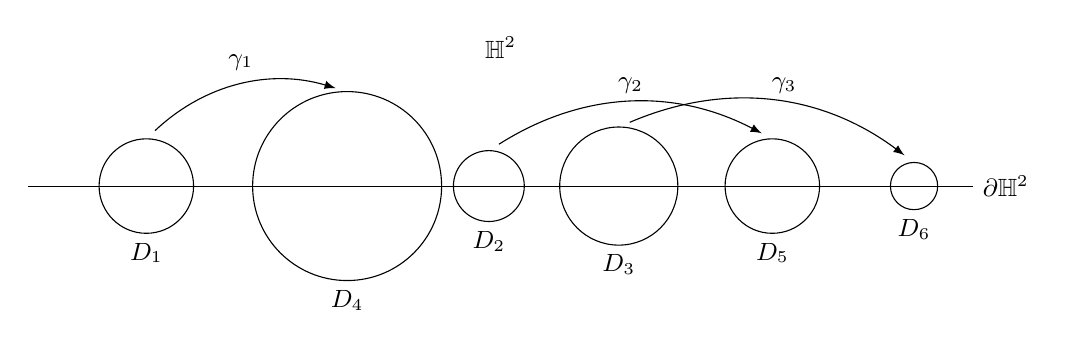
\begin{tikzpicture}[xscale=1.5, yscale=1.5]
\draw (-4,0) -- (4,0) node [right, font=\small]  {$  \partial \HH^2 $};
\draw (0,1) node [above, font=\small]  {$ \HH^2 $};
%disks plus labelling
\draw (-3,0) circle [radius = 0.4];
\draw (-1.3,0) circle [radius = 0.8];
\draw (-0.1,0) circle [radius = 0.3];
\draw (1,0) circle [radius = 0.5];
\draw (2.3,0) circle [radius = 0.4];
\draw (3.5,0) circle [radius = 0.2];
%labelling the disks
\draw (-3,-0.4) node[below,font=\small] {$ D_{1} $};
\draw (-1.3,-0.8) node[below,font=\small] {$ D_{4} $};
\draw (-0.1,-0.3) node[below,font=\small] {$ D_{2} $};
\draw (1,-0.5) node[below,font=\small] {$ D_{3} $};
\draw (2.3,-0.4) node[below,font=\small] {$ D_{5} $};
\draw (3.5,-0.2) node[below,font=\small] {$ D_{6} $};
%arrows between disks
%1 to 4
 \draw [arrow, bend left]  (-3,0.4) to (-1.3,0.8);
%2 to 5
 \draw [arrow, bend left]  (-0.1,0.3) to (2.3,0.4);
%3 to 6
 \draw [arrow, bend left]  (1,0.5) to (3.5,0.2);
%Labelling the isometries
 \draw (-2.2,0.9) node[above,font=\small] {$ \gamma_{1} $};
 \draw (1.1,0.7) node[above,font=\small] {$ \gamma_{2} $};
 \draw (2.4,0.7) node[above,font=\small] {$ \gamma_{3} $};
\end{tikzpicture}
\caption{A configuration of Schottky disks and isometries with $ m=3 $}
\end{figure}

A Fuchsian group $\Gamma$ is called \textit{elementary} if its limit set $\Lambda$ is a finite set. If $\Gamma$ is a Schottky group as above, then it is elementary if and only if $m=1,$ in which case $\Gamma\backslash \HH^2$ is a hyperbolic cylinder.

\textit{Throughout the rest of this paper we assume that $X=\Gamma\backslash \HH^2$ is a convex cocompact quotient where $\Gamma$ is a non-elementary Schottky group with Schottky data $D_1, \dots, D_{2m}$ and $\gamma_1, \dots, \gamma_{2m}$ as above. This assumption will not be repeated in the sequel.}


\subsection{Combinatorial notation for words}\label{sec:comNotation}
We will use a combinatorial notation for elements of the free group $\Gamma$, essentially following Dyatlov–Zworski \cite{DyZw18}.

\begin{itemize}
\setlength\itemsep{1em}

\item Let $\mathcal{A} = \{1, \dots, 2m\}$ be the alphabet. A word $\Aa = a_1 \cdots a_n$ is a string of letters $a_j \in \mathcal{A}$. Let $|\Aa|$ denote the length of the word, i.e., the number of letters in $\Aa.$
We introduce the empty word $\emptyset$ of length zero for technical reasons.

\item A word $\Aa = a_1 \cdots a_n$ is \textit{reduced} if $a_j \ne \overline{a_{j+1}}$ for all $1 \le j \le n-1$. Define $\mathcal{W}_n$ to be the set of reduced words of length $n$:
\[
\mathcal{W}_n = \left\{ a_1 \cdots a_n : a_j \in \mathcal{A},\, a_j \ne \overline{a_{j+1}} \right\}.
\]
Set $\mathcal{W}_0 = \{\emptyset\}$ and $\mathcal{W} = \bigsqcup_{n \ge 0} \mathcal{W}_n$. Also define $\mathcal{W}_{\ge m} = \bigsqcup_{n \ge m} \mathcal{W}_n$ and $\mathcal{W}^\circ = \mathcal{W}_{\ge 1}$.

\item For any word $\Aa$, define its reduced form $\mathsf{red}(\Aa) \in \mathcal{W}$ by repeatedly applying the rule $a \overline{a} = \emptyset$. Then $\gamma_\Aa = \gamma_{\mathsf{red}(\Aa)}$ in $\Gamma$.

\item For $\Aa = a_1 \cdots a_n \in \mathcal{W}^\circ$, write $\Aa' = a_1 \cdots a_{n-1}$. The set $\mathcal{W}$ forms a rooted tree with root $\emptyset$, and $\Aa'$ is the parent of $\Aa$.

\item For $\Aa, \Bb \in \mathcal{W}$, write $\Aa \to \Bb$ if either $\Aa = \emptyset$, $\Bb = \emptyset$, or both are non-empty and $a_n \ne \overline{b_1}$; in this case, the concatenation $\Aa\Bb$ is reduced.

\item Let $z\in \CC.$ We write $\Aa \to z$ if there exists $b \in \mathcal{A}$ such that $\Aa \to b$ and $z \in D_b$.

\item Define the mirror word $\overline{\Aa} = \overline{a_n} \cdots \overline{a_1}$.

\item Write $\Aa \prec \Bb$ if $\Aa$ is a prefix of $\Bb$, i.e., $\Bb = \Aa\Cc$ for some $\Cc \in \mathcal{W}$.

\item The map $\Aa = a_1 \cdots a_n \mapsto \gamma_\Aa = \gamma_{a_1} \cdots \gamma_{a_n}$ gives a bijection between reduced words and elements of $\Gamma$. Moreover:
\[
\gamma_{\Aa\Bb} = \gamma_\Aa \gamma_\Bb, \qquad \gamma_\Aa^{-1} = \gamma_{\overline{\Aa}}, \qquad \gamma_\Aa = \mathrm{id} \iff \Aa = \emptyset.
\]

\item For $\Aa = a_1 \cdots a_n \in \mathcal{W}^\circ$, define the disk $D_\Aa := \gamma_{\Aa'}(D_{a_n})$. Then:
\begin{enumerate}[(i)]
  \item If $\Aa \prec \Bb$, then $D_\Bb \subset D_\Aa$.
  \item If neither $\Aa \prec \Bb$ nor $\Bb \prec \Aa$, then $D_\Aa \cap D_\Bb = \emptyset$.
\end{enumerate}
Define the interval
\[
I_\Aa := D_\Aa \cap \mathbb{R},
\]
with length $|I_\Aa|$ equal to the diameter of $D_\Aa$. These intervals contract exponentially: there are constants $C > 0$ and $0 < \theta < 1$ such that
\begin{equation}\label{eq:unifContraction}
|I_\Aa| \le C \theta^{|\Aa|} \quad \text{for all } \Aa \in \mathcal{W}^\circ.
\end{equation}

\item Define the union sets:
\[
D = \bigsqcup_{a \in \mathcal{A}} D_a, \qquad I = \bigsqcup_{a \in \mathcal{A}} I_a.
\]

\item The limit set of $\Gamma$ is given by
\[
\Lambda = \bigcap_{n \ge 1} \bigsqcup_{\Aa \in \mathcal{W}_n} I_\Aa \subset \mathbb{R}.
\]
\end{itemize}

\subsection{The standard transfer operator}\label{sec:classicalTransfOper}
Given a non-empty, open set $\Omega \subset \CC$, the \textit{Bergman space} $H^2(\Omega)$ is the Hilbert space of square-integrable holomorphic functions in $\Omega$:
\begin{equation}\label{defi_bergman}
H^2(\Omega) := \left\{ f \colon \Omega \to \CC \;\text{holomorphic} \;\middle|\; \|f\| < \infty \right\},
\end{equation}
with norm
\[
\|f\|^2 := \int_\Omega |f(z)|^2 \, \mathrm{dvol}(z),
\]
where $\mathrm{vol}$ is the standard two-dimensional Lebesgue measure on $\CC$.

Let $D = \bigsqcup_{a \in \mathcal{A}} D_a \subset \CC$ be the union of the Schottky disks introduced in Section~\ref{sec:SchottkyGroups}. We define the holomorphic family of \textit{transfer operators} $\mathcal{L}_s \colon H^2(D) \to H^2(D)$, parametrized by $s \in \CC$, via
\begin{equation}\label{transf_defi}
\mathcal{L}_s f(z) := \sum_{\substack{a \in \mathcal{A} \\ a \to b}} \gamma_a'(z)^s f(\gamma_a(z)), \quad \text{for } z \in D_b.
\end{equation}
Since $\gamma_a'(z) > 0$ for $z \in I_b$, the complex power $\gamma_a'(z)^s$ is holomorphic and unambiguously defined. Explicitly,
\begin{equation}\label{defi:principal_branch}
\gamma_a'(z)^s = \exp\left( s \mathbb{L}(\gamma_a'(z)) \right), \quad \text{where} \quad \mathbb{L}(z) := \log|z| + \mathrm{arg}(z),
\end{equation}
and $\mathrm{arg} \colon \CC \setminus (-\infty, 0] \to (-\pi, \pi)$ is the principal branch of the argument.

The transfer operator $\mathcal{L}_s$ appears, for instance, in \cite[Chapter~15]{Borthwick_book}. We have the following key identity:

\begin{prop}[Fredholm determinant identity]\label{prop:Fredholm_identity}
For all $s \in \CC$, the operator $\mathcal{L}_s$ is trace class on $H^2(D)$, and
\begin{equation}\label{Fredholm_identity_equation}
Z_\Gamma(s) = \det(1 - \mathcal{L}_s).
\end{equation}
\end{prop}

As a consequence, $s \in \CC$ is a resonance of $X = \Gamma \backslash \HH^2$ if and only if $\mathcal{L}_s$ has $1$ as an eigenvalue with some non-zero eigenfunction $f \in H^2(D)$.

\subsection{Partitions and refined transfer operators}\label{sec:partRefOp}
In this paper, we work with \textit{refined} transfer operators. These are generalizations of the standard transfer operator $\mathcal{L}_s$ introduced by Dyatlov–Zworski \cite{DyZw18}.

Given any finite subset $Z \subset \mathcal{W}$, define:
\begin{itemize}
  \item $Z' := \{ \Aa' : \Aa \in Z \}$,
  \item $\overline{Z} := \{ \overline{\Aa} : \Aa \in Z \}$.
\end{itemize}
For any $Z \subset \mathcal{W}$ we define an operator $\mathcal{L}_{Z,s} \colon H^2(D) \to H^2(D)$ by
\begin{equation}\label{generalizedOp}
\mathcal{L}_{Z,s}f(z) := \sum_{\substack{\Aa \in (\overline{Z})' \\ \Aa \to b}} \gamma_{\Aa}'(z)^s f(\gamma_{\Aa}(z)), \quad \text{for } z \in D_b.
\end{equation}
Note that for $Z=\mathcal{W}_2$ we have $\mathcal{L}_{Z,s} = \mathcal{L}_{s}.$

The key definition here is


\begin{defi}[Partitions]
A finite set $Z \subset \mathcal{W}^\circ$ is called a \textit{partition} if there exists $N \in \mathbb{N}$ such that every $\Aa \in \mathcal{W}$ with $|\Aa| \ge N$ has a \textit{unique} prefix $\Bb \in Z$, i.e., $\Bb \prec \Aa$. Equivalently, $Z$ is a partition if we have the \textit{disjoint} union
\[
\Lambda = \bigsqcup_{\Bb \in Z} (I_{\Bb} \cap \Lambda).
\]
\end{defi}

Trivial examples for partitions include $\mathcal{W}_n$ for $n \ge 2$, in which case we have $\mathcal{L}_{\mathcal{W}_n, s} = \mathcal{L}_s^{n - 1}$.
The partitions relevant in this paper are the sets of words discretizing to some resolution $\tau > 0$:
$$
Z(\tau):= \{ \Aa\in \mathcal{W}^{\circ} : \vert I_{\Aa}\vert \le  \tau < \vert I_{\Aa'}\vert \}.
$$
The notion of partitions as well as the partitions $Z(\tau)$ were originally introduced in \cite{DyZw18}. Next, we define the \textit{$\tau$-refined transfer operator} $\mathcal{L}_{\tau,s}$ as
\begin{equation}\label{defiRefinedTO}
\mathcal{L}_{\tau,s}f(z) := \mathcal{L}_{Z(\tau),s}f(z)= \sum_{\substack{ \Aa\in Y(\tau) \\ \Aa\to b}} \gamma_{\Aa}'(z)^s f(\gamma_{\Aa} (z))\ \mathrm{if}\ z\in D_b,
\end{equation}
where we put
\begin{equation}\label{defi:Y}
Y(\tau) := \overline{Z(\tau)}'.
\end{equation}

The operator $\mathcal{L}_{\tau,s}$ is well-defined if $Y(\tau) \subset \mathcal{W}^\circ$, which holds provided $\tau$ is sufficiently small so that $Z(\tau) \subset \mathcal{W}_{\ge 2}$.

The main reason for using this special family of operators is that we can control the size of the set $Y(\tau)$ as well as the absolute values of the derivatives $\gamma_{\Aa}'$ for $\Aa\in Y(\tau)$ in a uniform way, see Lemma \ref{lem:YZ} below. This is what enables us to obtain explicit exponents in Theorem \ref{main_thm}.



The fundamental fact about partitions is

\begin{lemma}\label{lem:partEigen}
Let $Z \subset \mathcal{W}_{\ge 2}$ be a partition. Then there exists a holomorphic family of trace class operators $T_{Z,s}$ such that
\begin{equation}\label{factWithTraceCLass}
1 - \mathcal{L}_{Z,s} = (1 + T_{Z,s})(1 - \mathcal{L}_s).
\end{equation}
In particular,
\begin{equation}\label{detPartitions}
\det(1 - \mathcal{L}_{Z,s}) = \det(1 + T_{Z,s}) \cdot Z_\Gamma(s).
\end{equation}
\end{lemma}

\begin{remark}
Lemma~\ref{lem:partEigen} extends Lemma~2.4 from Dyatlov--Zworski \cite{DyZw18}, which states that any $1$-eigenfunction of $\mathcal{L}_s$ is also a $1$-eigenfunction of $\mathcal{L}_{Z,s}$. Our result is stronger: it shows that the Fredholm determinant $\det(1 - \mathcal{L}_{Z,s})$ is a holomorphic multiple of the Selberg zeta function $Z_\Gamma(s)$. In particular, every zero of $Z_\Gamma(s)$ is also a zero of $\det(1 - \mathcal{L}_{Z,s})$, with at least the same multiplicity. The proof is a straightforward adaptation of the argument in \cite{DyZw18}.
\end{remark}


\begin{proof}
The identity in \eqref{detPartitions} follows from taking determinants on both sides of \eqref{factWithTraceCLass} and then applying Proposition \ref{prop:Fredholm_identity}.For the latter, we argue by induction on $\sum_{\textbf{b}\in Z'} \vert \textbf{b}\vert$. If $Z = \mathcal{W}_2$ then $\mathcal{L}_{Z,s} = \mathcal{L}_s$, so \eqref{factWithTraceCLass} holds true with $T_{\mathcal{W}_2,s} = 0$. If $Z \neq \mathcal{W}_2$, choose a word $\textbf{d}c\in Z$ of maximal length, where $\textbf{d}\in \mathcal{W}^\circ$ and $c\in \mathcal{A}$. 
\begin{figure}[h!]
\centering
\begin{forest}
for tree={
    draw,
    rectangle,
    rounded corners,
    align=center,
    edge={-}
}
[$\emptyset$ 
    [1,
        [11, fill=lightgray]
        [12, 
	        [121, fill=lightgray, scale=0.7]
    	    [122, fill=lightgray, scale=0.7]
        	[123, fill=lightgray, scale=0.7]
        ]
        [14, fill=lightgray]
    ] 
    [2 
        [21, fill=lightgray]
        [22, fill=lightgray]
        [23, fill=lightgray]
    ]
    [3 
        [32, fill=black, text=white
	        [321, fill=lightgray, scale=0.6]
    	    [323, fill=lightgray, scale=0.6]
        	[323, fill=lightgray, scale=0.6]        
        ]
        [33, fill=lightgray]
        [34,
	        [341, fill=lightgray, scale=0.6]
    	    [343, fill=lightgray, scale=0.6]
        	[344, fill=lightgray, scale=0.6]                
        ]
    ] 
    [4 
        [41, fill=lightgray]
        [43, fill=lightgray]
        [44,
        	[441, fill=lightgray, scale=0.7]
    	    [443, fill=lightgray, scale=0.7]
        	[444, fill=lightgray, scale=0.7]        
        ]
    ]
]
\end{forest}
\caption{An example of a partition $Z$, with elements of $Z$ shaded grey in the tree of words. The solid black word is one possible choice of $\textbf{d}$ in the proof of Lemma \ref{lem:partEigen}.}
\label{fig:my-tree}
\end{figure}
Then $Z$ has the form (cf. Figure~\ref{fig:my-tree})
\begin{equation}\label{eq:newform}
Z = (Z_0 \smallsetminus \{\textbf{d}\}) \sqcup \{ \textbf{d}a : a \in \mathcal{A},\, \textbf{d} \to a \},
\end{equation}
where $Z_0$ is a partition containing $\textbf{d}$. By the inductive hypothesis, we have
\begin{equation}\label{indHyp}
1 - \mathcal{L}_{Z_0,s} = (1 + T_{Z_0,s})(1 - \mathcal{L}_s).
\end{equation}
We write $\mathcal{L}_{Z,s}$ as
\[
\mathcal{L}_{Z,s} = \sum_{\Aa \in (\overline{Z})'} \nu_{\Aa,s},
\]
where each $\nu_{\Aa,s} \colon H^2(D) \to H^2(D)$ is defined by
\[
\nu_{\Aa,s}(f)(z) :=
\begin{cases}
\gamma_\Aa'(z)^s f(\gamma_\Aa(z)) & \text{if } \Aa \to z, \\
0 & \text{otherwise}.
\end{cases}
\]
Using \eqref{eq:newform}, we write
\[
\mathcal{L}_{Z,s} = \mathcal{L}_{Z_0 \smallsetminus \{ \textbf{d} \},s} + \sum_{a \in \mathcal{A}} \nu_{\overline{\textbf{d}a}',s}.
\]
For each $a$ such that $\textbf{d} \to a$, observe that
\[
\overline{\textbf{d}a}' = \overline{a} \, \overline{\textbf{d}}',
\quad \text{and hence} \quad
\nu_{\overline{\textbf{d}a}',s} = \nu_{\overline{\textbf{d}}',s} \nu_{a,s}.
\]
Inserting this into the previous expression for $\mathcal{L}_{Z,s}$, we get
\begin{align*}
\mathcal{L}_{Z,s}
&= \mathcal{L}_{Z_0 \smallsetminus \{ \textbf{d} \},s} + \sum_{a \in \mathcal{A}} \nu_{\overline{\textbf{d}}',s} \nu_{a,s} \\
&= \mathcal{L}_{Z_0,s} - \nu_{\overline{\textbf{d}}',s} + \nu_{\overline{\textbf{d}}',s} \mathcal{L}_s \\
&= \mathcal{L}_{Z_0,s} - \nu_{\overline{\textbf{d}}',s}(1 - \mathcal{L}_s).
\end{align*}
Combining this with \eqref{indHyp}, we find
\[
1 - \mathcal{L}_{Z,s} = \left(1 + T_{Z_0,s} + \nu_{\overline{\textbf{d}}',s}\right)(1 - \mathcal{L}_s),
\]
which establishes the relation in \eqref{factWithTraceCLass} with
\begin{equation}\label{eq:recursion}
T_{Z,s} := T_{Z_0,s} + \nu_{\overline{\textbf{d}}',s}.
\end{equation}
Since both $T_{Z_0,s}$ and $\nu_{\overline{\textbf{d}}',s}$ are trace class, so is $T_{Z,s}$, completing the proof.
\end{proof}


\begin{remark}
Although not important for this paper, it is worth noting that repeated application of \eqref{eq:recursion} yields the identity
\[
T_{Z,s} = \mathcal{L}_{Z^\prec,s},
\]
where $Z^\prec$ denotes the set of all prefixes of words in $Z$:
\[
Z^\prec := \left\{ \textbf{b} \in \mathcal{W} \mid \exists\, \textbf{a} \in Z \text{ such that } \textbf{b} \prec \textbf{a} \right\}.
\]
In the tree representation of $\mathcal{W}$ (see Figure~\ref{fig:my-tree}), $Z^\prec$ corresponds to all ancestors of $Z$. In the specific case $Z = \mathcal{W}_{n+1}$, we have
\[
Z^\prec = \bigcup_{1 \le m \le n} \mathcal{W}_m,
\]
and Equation \eqref{factWithTraceCLass} becomes the standard identity
\[
1 - \mathcal{L}_s^n = (1 + \mathcal{L}_s + \cdots + \mathcal{L}_s^{n-1})(1 - \mathcal{L}_s).
\]
\end{remark}

It is straightforward to generalize Lemma~\ref{lem:partEigen} to products:


\begin{lemma}\label{lem:holomMultiple}
Let $k \ge 1$ and let $Z_1, \dots, Z_k \subset \mathcal{W}_{\ge 2}$ be a collection of partitions. Then there exists a holomorphic family of trace class operators $T_s$ (depending on $Z_1, \dots, Z_k$) such that
\[
1 - \mathcal{L}_{Z_1,s} \cdots \mathcal{L}_{Z_k,s} = (1 + T_s)(1 - \mathcal{L}_s).
\]
Consequently,
\[
\det\left(1 - \mathcal{L}_{Z_1,s} \cdots \mathcal{L}_{Z_k,s}\right)
\]
is a holomorphic multiple of $Z_\Gamma(s)$.
\end{lemma}

\begin{proof}
We proceed by induction on $k$. For $k = 1$, the statement is Lemma~\ref{lem:partEigen}. Suppose $k > 1$. By the inductive hypothesis, there exists a holomorphic family of trace class operators $\widetilde{T}_s$ such that
\[
1 - \mathcal{L}_{Z_1,s} \cdots \mathcal{L}_{Z_{k-1},s} = (1 + \widetilde{T}_s)(1 - \mathcal{L}_s).
\]
Applying Lemma~\ref{lem:partEigen} to $\mathcal{L}_{Z_k,s}$, we have
\[
1 - \mathcal{L}_{Z_k,s} = (1 + T_{Z_k,s})(1 - \mathcal{L}_s).
\]
Using this, we obtain
\begin{align*}
1 - \mathcal{L}_{Z_1,s} \cdots \mathcal{L}_{Z_k,s}
&= 1 - \left(1 - (1 + \widetilde{T}_s)(1 - \mathcal{L}_s)\right) \mathcal{L}_{Z_k,s} \\
&= 1 - \left(1 - (1 + \widetilde{T}_s)(1 - \mathcal{L}_s)\right) \left(1 - (1 + T_{Z_k,s})(1 - \mathcal{L}_s)\right) \\
&= \left[(1 + \widetilde{T}_s) + (1 + T_{Z_k,s}) - (1 + \widetilde{T}_s)(1 - \mathcal{L}_s)(1 + T_{Z_k,s})\right](1 - \mathcal{L}_s).
\end{align*}
Since sums and products of trace class operators remain trace class, the bracketed expression defines an operator of the form $1 + T_s$ for some trace class $T_s$, which depends holomorphically on $s \in \CC$.
\end{proof}


\subsection{Bounds for Schottky groups}\label{sec:boundsForDeriv}
We now record standard estimates for elements of Schottky groups. We introduce new notation following Magee--Naud \cite{NaudMagee}. For each $a \in \mathcal{A}$, fix a point $o_a \in I_a$. These are treated as fixed reference points. For any $\textbf{a} \in \mathcal{W}^\circ$, define
\[
o_{\textbf{a}} := o_b,
\]
for some $b \in \mathcal{A}$ with $\textbf{a} \to b$, and let $o_\emptyset$ be any point in $D$. Then for $\textbf{a} \in \mathcal{W}$, define
\begin{equation}\label{defi:Upsilon}
\Upsilon_{\textbf{a}} := \gamma_{\textbf{a}}'(o_{\textbf{a}}).
\end{equation}
From \cite{NaudMagee}, we have the following estimates:

\begin{lemma}[Bounds for derivatives]\label{lem:boundsderivatives}
The following estimates hold with implied constants depending only on $\Gamma$:
\begin{enumerate}[(i)]
\item \label{part:ups} For all $b \in \mathcal{A}$ and all $z \in D_b$ with $\Aa \to b$, we have
\[
|\gamma'_{\Aa}(z)| \asymp \vert I_\Aa\vert \asymp \Upsilon_{\Aa}.
\]

\item For all $\Aa \in \mathcal{W}^\circ$, we have
\[
\Upsilon_{\Aa'} \asymp \Upsilon_{\Aa}.
\]

\item \label{part:mirrorEst} For all $\Aa \in \mathcal{W}^\circ$, we have
\[
\Upsilon_{\overline{\Aa}} \asymp \Upsilon_{\Aa}.
\]

\item \label{part:almostMultip} For all $\Aa, \Bb \in \mathcal{W}^\circ$ with $\Aa \to \Bb$, we have
\[
\Upsilon_{\Aa\Bb} \asymp \Upsilon_{\Aa} \Upsilon_{\Bb}.
\]
\end{enumerate}
\end{lemma}

\begin{lemma}[Estimates for $Z(\tau)$ and $Y(\tau)$]\label{lem:YZ}
For all $\tau > 0$, the following estimates hold with constants depending only on $\Gamma$:
\begin{enumerate}[(i)]
\item For all $\Aa \in Z(\tau)$ and all $\Aa \in Y(\tau)$, we have
\[
\Upsilon_{\Aa} \asymp \tau.
\]

\item \label{cardinalityzy} The cardinalities satisfy
\[
|Z(\tau)| \asymp |Y(\tau)| \asymp \tau^{-\delta}.
\]

\item \label{lengthsofwords} For all $\Aa \in Z(\tau)$ and all $\Aa \in Y(\tau)$, we have
\[
|\Aa| \asymp \log(\tau^{-1}).
\]
\end{enumerate}
\end{lemma}

\begin{proof}
The estimates for $Z(\tau)$ appear in \cite{Bourgain_Dyatlov, NaudMagee}. The bounds for $Y(\tau)$ follow from those for $Z(\tau)$ and Lemma~\ref{lem:boundsderivatives}.
\end{proof}

Also helpful is the following lemma:

\begin{lemma}\label{lem:cardsets}
There exists a constant \( C > 0 \), depending only on \( \Gamma \), such that for all \( \tau > 0 \), we have
\[
\#\left\{ \Aa \in \mathcal{W} : \Upsilon_{\Aa} > \tau \right\} \le C(\tau^{-\delta} + 1).
\]
\end{lemma}

\begin{proof}
By \cite[Lemma~10]{CalMag25}, the Frobenius norm of \( \gamma_{\Aa} \) for all \( \Aa \in \mathcal{W} \) satisfies
\[
\Vert \gamma_{\Aa} \Vert \asymp_\Gamma \vert I_\Aa\vert^{-1/2} \asymp_\Gamma \Upsilon_\Aa^{-1/2}.
\]
Moreover, we have the well-known lattice point estimate for all \( x > 0 \) (see for instance \cite[Theorem~14.22]{Borthwick_book}):
\[
\#\left\{ \gamma \in \Gamma : \Vert \gamma \Vert < x \right\} \ll x^{2\delta} + 1.
\]
Combining these two estimates yields the lemma.
\end{proof}





\subsection{Refined function spaces}\label{sec:refinedFuncti}
In this paper, we adopt the approach of Guillop\'{e}--Lin–Zworski \cite{GLZ}. The idea is to let transfer operators act on \textit{refined} function spaces. To construct these spaces, fix a small parameter $h > 0$ and consider the real $h$-neighbourhood of the limit set:
\begin{equation}\label{defi:realhneighbourhood}
\Lambda(h) := \Lambda + (-h, h).
\end{equation}
The following structural result is known from \cite{GLZ}; see also \cite[Lemma~15.14]{Borthwick_book}.

\begin{lemma}[Structure of $\Lambda(h)$]\label{lem:structureLambdah}
There exists a constant $C > 0$ such that for all sufficiently small $h > 0$, the set $\Lambda(h)$ is a union of at most $C h^{-\delta}$ connected components, each with diameter at most $Ch$.
\end{lemma}
We can therefore write
\begin{equation}\label{LambdaUnion}
\Lambda(h) = \bigsqcup_{l = 1}^{N(h)} I_l(h),
\end{equation}
where $I_l(h) \subset \mathbb{R}$ are real intervals with mutually disjoint closures, satisfying $|I_l(h)| \le Ch$ and $N(h) \le C h^{-\delta}$. Let $D_l(h) \subset \CC$ be the unique open Euclidean disk centered on the real line such that $D_l(h) \cap \mathbb{R} = I_l(h)$. Define the refined domain:
\begin{equation}\label{defi:omega(h)}
\Omega(h) := \bigsqcup_{l = 1}^{N(h)} D_l(h).
\end{equation}
For each $b \in \mathcal{A}$, let
\[
\Omega_b(h) := \Omega(h) \cap D_b.
\]
Given a partition $Z \subset \mathcal{W}_{\ge 2}$, we define the refined transfer operator $\mathcal{L}_{Z,s} \colon H^2(\Omega(h)) \to H^2(\Omega(h))$ by
\begin{equation}\label{refOpRefSpace}
\mathcal{L}_{Z,s}f(z) := \sum_{\substack{\Aa \in \overline{Z}' \\ \Aa \to b}} \gamma'_{\Aa}(z)^s f(\gamma_{\Aa}(z)), \quad \text{for } z \in \Omega_b(h).
\end{equation}
This definition is similar to \eqref{generalizedOp}, except that here we impose a restriction on the range of $z$. 


The following lemma is crucial. 

\begin{lemma}[Contraction in $\Omega(h)$]\label{lem:contractionInH}
There exist $N_0 \in \mathbb{N}$ and $h_0 > 0$, depending only on $\Gamma$, such that for all $h \in (0, h_0)$, all $b \in \mathcal{A}$, all $z \in \Omega_b(h)$, and all $\Aa \in \mathcal{W}_{\ge N_0}$ with $\Aa \to b$, we have
\[
\mathrm{dist}(\gamma_{\Aa}(z), \partial \Omega(h)) > h/2.
\]
In other words, $\gamma_{\Aa}(\Omega_b(h)) \subset \Omega(h/2)$.
\end{lemma}

\begin{proof}
The argument is the same as in \cite[Lemma~3.2]{Naud14}. Fix $b \in \mathcal{A}$, $z \in \Omega_b(h)$, and $\Aa \in \mathcal{W}^\circ$ with $\Aa \to b$.  It suffices to show $\gamma_{\Aa}(z) \in \Omega(h/2)$ for $|\Aa|$ large.

Since $\Omega(h)$ is a union of Euclidean disks centered on $\mathbb{R}$ and $\gamma_{\Aa}$ is a Möbius transformation, we may assume $z \in \Lambda(h) \cap I_b$. Then $z$ is $h$-close to some $p \in \Lambda \cap I_b$, so $|z - p| \le h$. By uniform contraction \eqref{eq:unifContraction}, there are constants $C > 0$ and $0 < \theta < 1$ such that
\[
|\gamma_{\Aa}(z) - \gamma_{\Aa}(p)| \le C \theta^{|\Aa|} h.
\]
Choosing $N_0$ large enough (and independently of $h$) shows that if $|\Aa| \ge N_0$, then $|\gamma_{\Aa}(z) - \gamma_{\Aa}(p)| \le h/2$. Since $\Lambda$ is $\Gamma$-invariant, $\gamma_{\Aa}(p) \in \Lambda$, implying that $\mathrm{dist}(\gamma_{\Aa}(z), \Lambda) \le h/2.$ Thus, $\gamma_{\Aa}(z) \in \Omega(h/2)$, as required.
\end{proof}

A direct consequence of this is

\begin{lemma}[Well-defined action on refined space]\label{lem:welldefinedness}
Let $N_0 \in \mathbb{N}$ and $h_0 > 0$ be as in Lemma~\ref{lem:contractionInH}. For every finite set $Z \subset \mathcal{W}_{\ge N_0}$ and every $h \in (0, h_0)$, the operator
\begin{equation}\label{defi:refTOonRefS}
\mathcal{L}_{Z,s} \colon H^2(\Omega(h)) \to H^2(\Omega(h)), \quad s \in \CC
\end{equation}
defined by Equation~\eqref{refOpRefSpace}, is well-defined and of trace class.

Moreover, there exists $\tau_0 > 0$ such that for all $\tau \in (0, \tau_0)$ and all $h \in (0, h_0)$, the estimate
\[
\mathrm{dist}(\gamma_{\Aa}(z), \partial \Omega(h)) > h/2
\]
holds for all $b \in \mathcal{A}$ and all $\Aa \in Y(\tau)$ with $\Aa \to b$. Consequently, the $\tau$-refined operator
\begin{equation}\label{defi:refTOonRefS_2}
\mathcal{L}_{\tau,s} \colon H^2(\Omega(h)) \to H^2(\Omega(h)), \quad s \in \CC
\end{equation}
is also well-defined and trace class.
\end{lemma}

\begin{proof}
The first part follows from Lemma~\ref{lem:contractionInH}. For the second, use Part~\eqref{lengthsofwords} of Lemma~\ref{lem:YZ} to choose $\tau_0 > 0$ such that $Y(\tau) \subset \mathcal{W}_{\ge N_0}$ for all $\tau \in (0, \tau_0)$. 
\end{proof}

\subsection{Some bounds for $\Omega(h)$}\label{sec:boundsForOmega}
We now record several key estimates concerning the refined set $\Omega(h)$.

\begin{lemma}[Volume bound]\label{lem:vol}
There exists a constant $C > 0$, depending only on $\Gamma$, such that for all $h > 0$, 
\[
\vol(\Omega(h)) \le C h^{-\delta + 2}.
\]
\end{lemma}

\begin{proof}
By Lemma~\ref{lem:structureLambdah}, $\Omega(h)$ is a disjoint union of at most $C h^{-\delta}$ disks, each of radius $\le C h$. Since each disk has area $\le \pi C^2 h^2$, this yields the stated bound.
\end{proof}

\begin{lemma}[Taylor expansion of $\mathbb{L}(\gamma_{\Aa}'(z))$ in $\Omega(h)$]\label{lem:taylor}
Let $\Aa \in \mathcal{W}^\circ$, $b \in \mathcal{A}$, and $z = x + i y \in \Omega(h)$ with $\Aa \to b$ and $z \in \Omega_b(h)$. Then, for all sufficiently small $h > 0$ in terms of $\Gamma$,
\[
\mathbb{L}(\gamma_{\Aa}'(z)) = \log(\gamma_{\Aa}'(x))  + O(h).
\]
where the implied constant depends only on $\Gamma$.
\end{lemma}

\begin{proof}
Write $\gamma_{\Aa}$ as a Möbius transformation:
\[
\gamma_{\Aa}(x) = \frac{a_{\Aa} x + b_{\Aa}}{c_{\Aa} x + d_{\Aa}}, \quad \gamma_{\Aa}'(x) = \frac{1}{(c_{\Aa} x + d_{\Aa})^2},
\]
where
\[
\gamma_{\Aa} = \pmat{a_{\Aa}}{b_{\Aa}}{c_{\Aa}}{d_{\Aa}}\in \mathrm{SL}_2(\R).
\]
Its $n$-th derivative satisfies
\[
\gamma_{\Aa}^{(n)}(x) = n! \left( \frac{1}{x_{\Aa} - x} \right)^{n - 1} \gamma_{\Aa}'(x), \quad \text{where } x_{\Aa} := \gamma_{\Aa}^{-1}(\infty) = -\frac{d_{\Aa}}{c_{\Aa}}.
\]
Since $z \in D_b$ and $x_{\Aa} \in D_{\overline{a}_n}$ (with $\overline{a}_n \neq b$), we have $|z - x_{\Aa}| \asymp_\Gamma 1 $. In particular, for all $x \in I_b$ and all $n \in \mathbb{N}$,
\begin{equation}\label{eq:bound_gamma_derivative}
|\gamma_{\Aa}^{(n)}(x)| \le n! C^n \gamma_{\Aa}'(x)
\end{equation}
for some $C > 0$ depending only on $\Gamma$.

Now let $z = x + i y \in \Omega_b(h)$, so $|y| = O(h)$. Taylor-expand $\gamma_{\Aa}'(z)$ around $iy$:
$$
\gamma_{\Aa}'(z)  = \gamma_{\Aa}'(x+iy)= \sum_{n=0}^\infty  \frac{\gamma_{\Aa}^{(n+1)}(x)}{n!} (iy)^n.
$$
Using \eqref{eq:bound_gamma_derivative}, we see that for all $h>0$ sufficiently small in terms of $\Gamma$,
\begin{equation}\label{afterTayloer}
\gamma_{\Aa}'(z) = \gamma_{\Aa}'(x) +  O( y  \gamma_{\Aa}'(x) ) = \gamma_{\Aa}'(x) \left(  1  +  O( y ) \right).
\end{equation}
Taking logarithms using the principal branch $\mathbb{L}$ from \eqref{defi:principal_branch}, we get
\[
\mathbb{L}(\gamma_{\Aa}'(z)) = \log(\gamma_{\Aa}'(x)) + \mathbb{L}\left(1 + O(y)\right),
\]
where we used the rule
$$
\mathbb{L}(az) = \log(a) + \mathbb{L}(z)
$$
for all $a\in \R_{>0}$ and $z\in \C\setminus (-\infty,0].$ Using the Taylor series $\mathbb{L}(1 + u) = u - \frac{u^2}{2} + \dots$ for $\vert u\vert < 1$, we conclude that for all $h>0$ sufficiently small in terms of $\Gamma$,
\[
\mathbb{L}(\gamma_{\Aa}'(z)) = \log(\gamma_{\Aa}'(x))  + O(h).
\]
\end{proof}

\begin{lemma}[Bound for complex powers of derivatives]\label{lem:crucial_estimate}
There exists $C > 0$, depending only on $\Gamma$, such that for all $b \in \mathcal{A}$, all $\Aa \in \mathcal{W}^\circ$ with $\Aa \to b$, and all $s = \sigma + i t \in \CC$ with $\sigma > 0$,
\[
z \in \Omega_b(h) \Longrightarrow |\gamma_{\Aa}'(z)^s| \le (C \Upsilon_{\Aa})^{\sigma} \exp(C h |t|).
\]
\end{lemma}

\begin{proof}
Let $z = x + i y \in \Omega_b(h)$. By Lemma~\ref{lem:taylor}, we have
\begin{align*}
\gamma_{\Aa}'(z)^s &= \gamma_{\Aa}'(z)^{\sigma} \exp\left(i t \mathbb{L}(\gamma_{\Aa}'(z))\right) \\
&= \gamma_{\Aa}'(z)^{\sigma} \exp\left(i t \left(\log(\gamma_{\Aa}'(x)) +  O(h)\right)\right).
\end{align*}
Taking absolute values yields
\[
|\gamma_{\Aa}'(z)^s| = |\gamma_{\Aa}'(z)|^{\sigma} \exp\left(O(h |t|)\right).
\]
Using $|y| = O(h)$, as well as $\gamma_{\Aa}'(z) \asymp \Upsilon_{\Aa}$ from Lemma~\ref{lem:boundsderivatives}, we conclude that
\[
|\gamma_{\Aa}'(z)^s| \le (C \Upsilon_{\Aa})^{\sigma} \exp(O(h |t|)),
\]
as claimed.
\end{proof}


\begin{remark}
\begin{itemize}
\item Lemma~\ref{lem:crucial_estimate} motivates the choice $h := |t|^{-1}$. This ensures that exponential terms of the form $\exp(C h |t|)$ remain uniformly bounded, allowing us to eliminate exponential growth in estimates. This is the key benefit of working in the refined function spaces $H^2(\Omega(h))$.

\item Lemma~\ref{lem:contractionInH} implies that for any finite collection of partitions $Z_1, Z_2, \dots, Z_k \subset \mathcal{W}_{\ge N_0}$, and for sufficiently small $h > 0$, the operator
\[
\mathcal{L}_{Z_1,s} \cdots \mathcal{L}_{Z_k,s} \colon H^2(\Omega(h)) \to H^2(\Omega(h))
\]
is well-defined and trace class. By carefully applying the Lefschetz fixed point formula (cf.~\cite[Lemma~15.9]{Borthwick_book}), one finds that the traces of its powers, and hence the Fredholm determinant $\det(1 - \mathcal{L}_{Z_1,s} \cdots \mathcal{L}_{Z_k,s})$, are independent of $h$. By Lemma~\ref{lem:holomMultiple}, this determinant equals $Z_\Gamma(s)$ times an entire function.
\end{itemize}
\end{remark}



\subsection{Properties of Bergman kernels}\label{sec:Bergman}
We now state some basic facts about Bergman kernels, which play a crucial role in our proof of Theorem~\ref{main_thm}. For an in-depth account of the material given here, see \cite{Krantz}.

Let $\Omega \subset \CC$ be a non-empty bounded (possibly disconnected) open set and let $H^2(\Omega)$ denote the associated Bergman space. As a closed subspace of $L^2(\Omega)$, $H^2(\Omega)$ is separable and admits an orthonormal basis $(\varphi_n)$. Thus, any $f \in H^2(\Omega)$ has the expansion
\[
f(z) = \sum_n c_n(f) \varphi_n(z), \quad
c_n(f) = \int_\Omega f(w) \overline{\varphi_n(w)} \dvol(w),
\]
with convergence absolute and uniform on compact subsets of $\Omega$.

By the Riesz representation theorem, there exists a unique function $\overline{B_\Omega(z,\cdot)} \in H^2(\Omega)$, called the \textit{Bergman reproducing kernel}, such that
\begin{equation}\label{berg:int}
f(z) = \int_\Omega B_\Omega(z,w) f(w) \dvol(w).
\end{equation}
We now derive an explicit expression for $B(z,w)$. For any fixed $z\in \Omega$, we can expand $\overline{B(z,w)}$ as follows:
\begin{equation}\label{berg:exp}
\overline{B(z,w)} = \sum_n c_n \varphi_n(w), 
\end{equation}
where 
\begin{equation}\label{berg:coeff}
c_n = \int_\Omega \overline{B(z,w)} \, \overline{\varphi_n(w)} \dvol(w).
\end{equation}
Inserting \eqref{berg:coeff} and \eqref{berg:exp} into \eqref{berg:int}, and using the uniqueness of the Bergman kernel, we obtain
\begin{equation}\label{eq:formulaBergmann}
B(z,w) = \sum_n \varphi_n(z) \overline{\varphi_n(w)},
\end{equation}
where the series is uniformly convergent on compact subsets of $ \Omega\times \Omega. $

\begin{lemma}[Basic properties of the Bergman kernel]\label{lem:BergmanBasicProp}
The following hold:
\begin{enumerate}[(i)]
\item \label{part:bergmanDiffComp} If $z, w$ lie in distinct connected components of $\Omega$, then $B_\Omega(z,w) = 0$.

\item \label{part:bergmanIneq} For all $z, w \in \Omega$,
\[
|B_\Omega(z,w)|^2 \le B_\Omega(z,z) B_\Omega(w,w).
\]

\item \label{part:bergmanVariational} Variational formula:
\[
B_\Omega(z,z) = \sup\left\{ |f(z)|^2 : f \in H^2(\Omega),\, \|f\| = 1 \right\}.
\]

\item \label{part:bergmanComp} Comparison property: If $z \in \Omega_1 \subset \Omega_2$, then
\[
B_{\Omega_2}(z,z) \le B_{\Omega_1}(z,z).
\]

\item \label{part:bergmanDisk} Explicit formula for disks:
For $D(z_0,r) := \{ z \in \CC : |z - z_0| < r \}$,
\[
B_{D(z_0,r)}(z,w) = \frac{2r^2}{\pi \left( r^2 - (z - z_0)(\overline{w} - \overline{z}_0) \right)^2}.
\]
\end{enumerate}
\end{lemma}

\begin{proof}
Parts \eqref{part:bergmanDiffComp}–\eqref{part:bergmanComp} follow from \eqref{eq:formulaBergmann} and the Cauchy–Schwarz inequality. To prove \eqref{part:bergmanDisk}, use the orthonormal basis
\[
\varphi_n(z) = \sqrt{\frac{n+1}{\pi r^2}} \left( \frac{z - z_0}{r} \right)^n, \quad n \in \mathbb{N}_0
\]
in \eqref{eq:formulaBergmann}.
\end{proof}

\begin{lemma}[Upper bound for the Bergman kernel]\label{lem:UpperBoundBergman}
Define
\[
\mathrm{dist}(z, \partial\Omega) := \inf_{z' \in \partial\Omega} |z - z'|.
\]
Then for all $z, w \in \Omega$,
\begin{equation}\label{UpperBoundBergmanineq}
|B_\Omega(z,w)| \le \frac{1}{\pi \, \mathrm{dist}(z, \partial\Omega) \, \mathrm{dist}(w, \partial\Omega)}.
\end{equation}
\end{lemma}

\begin{proof}
Choose radii $r_z < \mathrm{dist}(z, \partial\Omega)$ and $r_w < \mathrm{dist}(w, \partial\Omega)$ so that $D(z, r_z), D(w, r_w) \subset \Omega$. By parts \eqref{part:bergmanIneq}, \eqref{part:bergmanComp}, and \eqref{part:bergmanDisk} of Lemma~\ref{lem:BergmanBasicProp}, we estimate:
\[
|B_\Omega(z,w)|^2 \le B_\Omega(z,z) B_\Omega(w,w)
\le B_{D(z, r_z)}(z,z) B_{D(w, r_w)}(w,w)
\le \frac{1}{\pi r_z^2} \cdot \frac{1}{\pi r_w^2}.
\]
Taking square roots yields
\[
|B_\Omega(z,w)| \le \frac{1}{\pi r_z r_w}.
\]
Letting $r_z \nearrow \mathrm{dist}(z, \partial\Omega)$ and $r_w \nearrow \mathrm{dist}(w, \partial\Omega)$ proves the claim.
\end{proof}

\section{Proof of Main Theorem}\label{sec:proofMainThm}
This section is devoted to the proof of Theorem~\ref{main_thm}, and is divided into several parts. Recall that $X = \Gamma \backslash \HH^2$ is a convex cocompact hyperbolic surface, and that we fix a Schottky representation for $\Gamma$ as in Section~\ref{sec:SchottkyGroups}. Throughout, we use the notations introduced in Section~\ref{sec:prelim}.

\subsection{Separation lemma}\label{sec:separation}
We begin with a separation lemma adapted from \cite[Lemma~4.4]{JN}, reflecting the total discontinuity of the limit set $\Lambda$.

\begin{lemma}[Separation Lemma]\label{lem:separation}
There exist constants $\widetilde{C} > 0$ and $h_0 > 0$, depending only on $\Gamma$, such that for all $0 < h < h_0$ and $\tau \ge \widetilde{C} h$, the following holds:

For all $b \in \mathcal{A}$, all words $\Aa, \Bb \in Y(\tau)$ with $\Aa, \Bb \to b$, and all points $z_1, z_2 \in D_b$, we have:
\[
\gamma_{\Aa}(z_1),\, \gamma_{\Bb}(z_2) \text{ lie in the same connected component of } \Omega(h) \quad \Longrightarrow \quad \Aa = \Bb.
\]
\end{lemma}

\begin{proof}
Fix $b \in \mathcal{A}$, $\Aa, \Bb \in Y(\tau)$ with $\Aa, \Bb \to b$, and $z_1, z_2 \in D_b$. Suppose $\Aa \neq \Bb$, yet $\gamma_{\Aa}(z_1)$ and $\gamma_{\Bb}(z_2)$ lie in the same component of $\Omega(h)$. We aim for a contradiction when $\tau \ge \widetilde{C} h$ for some sufficiently large constant $\widetilde{C}$.

By Lemma~\ref{lem:structureLambdah}, each component of $\Omega(h)$ has diameter $\le Ch$, so
\begin{equation}\label{diamH}
|\gamma_{\Aa}(z_1) - \gamma_{\Bb}(z_2)| \le Ch.
\end{equation}

If the first letters of $\Aa$ and $\Bb$ differ, then $\gamma_{\Aa}(z_1)$ and $\gamma_{\Bb}(z_2)$ lie in distinct Schottky disks, hence
\[
|\gamma_{\Aa}(z_1) - \gamma_{\Bb}(z_2)| \ge K,
\]
where $K > 0$ is the minimal distance between two Schottky disks, contradicting \eqref{diamH} for small $h$. Hence, $\Aa$ and $\Bb$ must share a common prefix $\Cc \in \mathcal{W}^\circ$, and we write $\Aa = \Cc \Aa_1$, $\Bb = \Cc \Bb_1$. Assume $\Cc$ is as long as possible, so that the first letters of $\Aa_1$ and $\Bb_1$ differ. Then
\begin{equation}\label{ineq:largerK2}
|\gamma_{\Aa_1}(z_1) - \gamma_{\Bb_1}(z_2)| \ge K.
\end{equation}
Now, using the identity for any Möbius transformation $\gamma$,
\[
|\gamma(u) - \gamma(v)| = |\gamma'(u)|^{1/2} |\gamma'(v)|^{1/2} |u - v|,
\]
applied to $\gamma = \gamma_\Cc$ and $u = \gamma_{\Aa_1}(z_1)$, $v = \gamma_{\Bb_1}(z_2)$, we obtain together with Lemmas~\ref{lem:boundsderivatives} and \ref{lem:YZ}:
\begin{align*}
|\gamma_{\Aa}(z_1) - \gamma_{\Bb}(z_2)|
&= |\gamma_\Cc'(\gamma_{\Aa_1}(z_1))|^{1/2} |\gamma_\Cc'(\gamma_{\Bb_1}(z_2))|^{1/2} |\gamma_{\Aa_1}(z_1) - \gamma_{\Bb_1}(z_2)| \\
&\gg \Upsilon_\Cc \cdot |\gamma_{\Aa_1}(z_1) - \gamma_{\Bb_1}(z_2)| \\
&\gg \Upsilon_\Aa \cdot |\gamma_{\Aa_1}(z_1) - \gamma_{\Bb_1}(z_2)| \\
&\gg \tau \cdot |\gamma_{\Aa_1}(z_1) - \gamma_{\Bb_1}(z_2)|.
\end{align*}
We also used that $\Upsilon_\Cc \gg \Upsilon_\Aa$ for any prefix $\Cc \prec \Aa$. From \eqref{ineq:largerK2}, we conclude
\[
|\gamma_{\Aa}(z_1) - \gamma_{\Bb}(z_2)| \ge C_0 \tau,
\]
for some $C_0 > 0$. Combining this with \eqref{diamH} gives $\tau \le \frac{C}{C_0} h$, which contradicts the assumption $\tau \ge \widetilde{C} h$ if $\widetilde{C} > \frac{C}{C_0}$. Taking $\widetilde{C} = \frac{2C}{C_0}$ completes the proof.
\end{proof}

\subsection{The phase and its derivative}\label{sec:phaseder}
For all words $\Aa, \Bb \in \mathcal{W}^\circ$ and points $z \in D$, we define the \textit{phase} function
\begin{equation}\label{phase}
\Phi_{\Aa, \Bb}(z) := \overline{\mathbb{L}(\gamma_{\Bb}'(z))} -\mathbb{L}(\gamma_{\Aa}'(z)),
\end{equation}
where $\mathbb{L}$ is the complex logarithm as in \eqref{defi:principal_branch}. For all $s = \sigma + i t \in \CC$, this yields
\[
\gamma_{\Aa}'(z)^s \cdot \overline{\gamma_{\Bb}'(z)^s}
= \gamma_{\Aa}'(z)^{\sigma} \cdot \overline{\gamma_{\Bb}'(z)}^{\sigma} \cdot e^{-i t \Phi_{\Aa, \Bb}(z)}.
\]
For a word $\textbf{a}$ in $\mathcal{A} = \{1, \dots, 2m\}$, let $\mathsf{red}(\textbf{a}) \in \mathcal{W}$ be its reduced form, obtained by applying the rule $a\overline{a} = \emptyset$ for all $a\in \mathcal{A}$. Recall the definition of $\Upsilon_{\Aa}$ from \eqref{defi:Upsilon}, and define
\begin{equation}\label{Dab}
\mathcal{D}_{\Aa, \Bb} := \left( \frac{\Upsilon_{\Aa} \Upsilon_{\Bb}}{\Upsilon_{\mathsf{red}(\Aa \overline{\Bb})}} \right)^{1/2}.
\end{equation}
Consider the following cases:
\begin{itemize}
\item If $\Aa \to \overline{\Bb}$, then $\mathsf{red}(\Aa \overline{\Bb}) = \Aa \overline{\Bb}$ and $\Upsilon_{\Aa \overline{\Bb}} \asymp \Upsilon_{\Aa} \Upsilon_{\Bb}$, so $\mathcal{D}_{\Aa, \Bb} \asymp 1$.
\item If alternativerly $\Aa \not\to \overline{\Bb}$, then $\Aa \overline{\Bb}$ is no longer reduced, and $\mathcal{D}_{\Aa, \Bb}$ may be very small.
\item In the extreme case $\Aa = \Bb$, we have $\mathsf{red}(\Aa \overline{\Bb}) = \emptyset$ and $\Upsilon_{\emptyset} = 1$, so $\mathcal{D}_{\Aa, \Bb} \asymp \Upsilon_\Aa$.
\item In any case, we have
\begin{equation}\label{eq:uniformDab}
\mathcal{D}_{\Aa, \Bb} = O(1),
\end{equation}
uniformly in $\Aa, \Bb$.
\end{itemize}

We now prove the key estimate:

\begin{prop}[Phase derivatives]\label{prop:phaseDerivative}
Let $b \in \mathcal{A}$ and $\Aa, \Bb \in \mathcal{W}^\circ$ with $\Aa, \Bb \to b$ and $\Aa \ne \Bb$. Then
\[
\inf_{x \in I_b} |\Phi_{\Aa, \Bb}'(x)| \asymp_\Gamma \mathcal{D}_{\Aa, \Bb}.
\]
\end{prop}

For the remainder of this section, we write for each word $\Aa$:
$$
\gamma_{\Aa} = \pmat{a_{\Aa}}{b_{\Aa}}{c_{\Aa}}{d_{\Aa}}\in \mathrm{SL}_2(\R).
$$
We need the following simple but crucial observation:

\begin{lemma}\label{lem:matrixEntriesBound}
For all words $\Aa$ in $\mathcal{A}$,
\[
|c_{\Aa}| \asymp_\Gamma \Upsilon_{\mathsf{red}(\Aa)}^{-1/2}.
\]
\end{lemma}

\begin{proof}
Since $\gamma_{\Aa} = \gamma_{\mathsf{red}(\Aa)}$, we may assume $\Aa$ is reduced. For $b \in \mathcal{A}$ with $\Aa \to b$ and $z \in D_b$,
\[
\gamma_{\Aa}'(z) = \frac{1}{(c_{\Aa} z + d_{\Aa})^2}
= \frac{1}{c_{\Aa}^2 (z - x_{\Aa})^2}, \quad \text{where } x_{\Aa} = -\frac{d_{\Aa}}{c_{\Aa}}.
\]
As in the proof of Lemma~\ref{lem:taylor}, we have $|z - x_{\Aa}| \asymp_\Gamma 1$, so $|\gamma_{\Aa}'(z)| \asymp_\Gamma \frac{1}{c_{\Aa}^2}$. The claim now follows from Lemma~\ref{lem:boundsderivatives}.
\end{proof}

\begin{proof}[Proof of Proposition~\ref{prop:phaseDerivative}]
Fix $b \in \mathcal{A}$, $x \in I_b$, and distinct $\Aa, \Bb \in \mathcal{W}^\circ$ with $\Aa, \Bb \to b$. Direct calculation yields
\begin{equation}\label{firstDer}
\Phi_{\Aa, \Bb}'(x) = 2\left( \frac{c_{\Bb}}{c_{\Bb} x + d_{\Bb}} - \frac{c_{\Aa}}{c_{\Aa} x + d_{\Aa}}  \right)
= 2 \cdot \frac{c_{\Bb} d_{\Aa} - c_{\Aa} d_{\Bb}}{(c_{\Aa} x + d_{\Aa})(c_{\Bb} x + d_{\Bb})}.
\end{equation}
Therefore,
\[
|\Phi_{\Aa, \Bb}'(x)| = 2 |c_{\Aa} d_{\Bb} - c_{\Bb} d_{\Aa}| \cdot |\gamma_{\Aa}'(x)|^{1/2} |\gamma_{\Bb}'(x)|^{1/2}.
\]
By Lemma~\ref{lem:boundsderivatives},
\[
|\Phi_{\Aa, \Bb}'(x)| \asymp_\Gamma |c_{\Aa} d_{\Bb} - c_{\Bb} d_{\Aa}| \cdot \Upsilon_{\Aa}^{1/2} \Upsilon_{\Bb}^{1/2}.
\]
Note that
\[
\gamma_{\Aa \overline{\Bb}} = \gamma_{\Aa} \gamma_{\Bb}^{-1} =
\begin{pmatrix}
\ast & \ast \\
c_{\Aa} d_{\Bb} - c_{\Bb} d_{\Aa} & \ast
\end{pmatrix},
\]
so by Lemma~\ref{lem:matrixEntriesBound},
\[
|c_{\Aa} d_{\Bb} - c_{\Bb} d_{\Aa}| \asymp_\Gamma \Upsilon_{\mathsf{red}(\Aa \overline{\Bb})}^{-1/2}.
\]
Therefore,
\[
|\Phi_{\Aa, \Bb}'(x)| \asymp_\Gamma \frac{\Upsilon_{\Aa}^{1/2} \Upsilon_{\Bb}^{1/2}}{\Upsilon_{\mathsf{red}(\Aa \overline{\Bb})}^{1/2}} = \mathcal{D}_{\Aa, \Bb},
\]
as claimed.
\end{proof}



\subsection{Averaged oscillatory integrals}\label{sec:averoscint}
Let $\varphi \in C^\infty(\mathbb{R})$ be a non-negative bump function with $\mathrm{supp}(\varphi) = [-2, 2]$ and $\varphi \equiv 1$ on $[-1, 1]$. Define
\[
\varphi_{T,H}(t) := \frac{1}{H}\, \varphi\left( \frac{t - T}{H} \right).
\]
Define the Fourier transform as usual by
\[
\widehat{\varphi}(\xi) := \int_{-\infty}^\infty \varphi(t)\, e^{-it\xi}\, dt.
\]
The aim of this section is to establish

\begin{prop}[Key bound for averaged oscillatory integrals]\label{prop:FOURIER} Let $\varphi_{T,H}$ be as above. There exists $T_0 = T_0(\Gamma) > 0$ such that for all $T \ge T_0$, $\eta > 0$, $T^\eta \le H \le T$, $b \in \mathcal{A}$, and $\Aa, \Bb \in \mathcal{W}^\circ$ with $\Aa, \Bb \to b$, all measurable $f \colon D \to \CC$, and all $\epsilon > 0$, the following holds with $h := \frac{1}{T}$:
\[
\left\vert \int_{\Omega_b(h)} \widehat{\varphi_{T,H}}\left(\Phi_{\Aa,\Bb}(z)\right) f(z)\, \dvol(z) \right\vert \ll_{\epsilon,\eta,\Gamma} 
\begin{cases}
h^{-\delta + 2} \Vert f \Vert_{\infty, \Omega_b(h)} & \text{if } \Aa = \Bb, \\[0.5em]
h^{-\delta + 2} \mathcal{D}_{\Aa, \Bb}^{-\delta} H^{-\delta + \epsilon} \Vert f \Vert_{\infty, \Omega_b(h)} & \text{if } \Aa \neq \Bb.
\end{cases}
\]
Here, $\mathcal{D}_{\Aa, \Bb}$ is defined as in \eqref{Dab}, and
\[
\Vert f \Vert_{\infty, \Omega_b(h)} := \sup_{z \in \Omega_b(h)} \vert f(z) \vert.
\]
\end{prop}


Recall that $\Lambda(h)$ is the real $h$-neighbourhood of the limit set as defined in \eqref{defi:realhneighbourhood}. Before proving Proposition \ref{prop:FOURIER}, we need a bound on the size of $\Lambda(h)$ intersected with small intervals:

\begin{lemma}\label{lem:boundInSmallIntervals}
There exists a constant $C > 0$, depending only on $\Gamma$, such that for every $x_0 \in I = \bigsqcup_{a \in \mathcal{A}} I_a$ and all $\nu, h > 0$, we have
\[
|\Lambda(h) \cap [x_0 - \nu, x_0 + \nu]| \le C h \left(1 + \frac{\nu}{h} \right)^\delta,
\]
where $\vert \cdot\vert$ denotes the Lebesgue measure.
\end{lemma}

\begin{proof}
For each $p \in I$, define $I(p; h) := [p - h, p + h]$. The set $\Lambda(h) \cap I(x_0;\nu) $ consists of all points $x\in I(x_0;\nu)$ for which there exists some $p\in \Lambda$ such that $\vert x-p\vert \leqslant h$. In this case, the triangle inequality implies that $p\in I(x_0; \nu + h).$ It follows that family of intervals $\{ I(p; h) : p \in \Lambda \cap I(x_0;  \nu + h) \}$ covers $\Lambda(h) \cap I(x_0; \nu)$. Observe that each of these intervals satisfies
\begin{equation}\label{eq:intervalContainment}
I(p; h) \subset I(x_0; \nu + 2h).
\end{equation}
By compactness, there exists a finite subcover $\{I(p_j; h)\}_{j=1}^k$. Applying the basic covering lemma yields a disjoint subcollection $\{I(q_j; h)\}_{j=1}^m$ of these intervals such that the enlarged intervals $\{I(q_j; 3h)\}_{j=1}^m$ cover $\Lambda(h) \cap I(x_0; \nu)$.

Let $\mu$ be the Patterson–Sullivan measure associated with $\Gamma$ (see \cite[Chapter~14]{Borthwick_book}). Since the intervals $I(q_j; h)$ are disjoint and each is contained in $I(x_0; \nu + 2h)$ by \eqref{eq:intervalContainment}, we have
\begin{equation}\label{eq:disjointness}
\sum_{j=1}^m \mu(I(q_j; h)) \le \mu(I(x_0; \nu + 2h)).
\end{equation}
By \cite[Lemma~14.13]{Borthwick_book}, for all $p \in \Lambda$,
\begin{equation}\label{eq:measGrowth}
\mu(I(p; h)) \asymp h^\delta,
\end{equation}
uniformly in $p$. Furthermore, since $\mu(I(x_0; \nu + 2h)) > 0$, the interval $I(x_0; \nu + 2h)$ intersects $\Lambda$, so there exists $p' \in \Lambda$ with $I(x_0; \nu + 2h) \subset I(p'; 2(\nu + 2h))$, giving
\begin{equation}\label{eq:measGrowth2}
\mu(I(x_0; \nu + 2h)) \le \mu( I(p'; 2(\nu + 2h))) \ll (\nu + h)^\delta.
\end{equation}
Combining \eqref{eq:measGrowth}, \eqref{eq:measGrowth2}, and \eqref{eq:disjointness}, the number of disjoint intervals is bounded by
\[
m \ll \frac{(\nu + h)^\delta}{h^\delta} = \left(1 + \frac{\nu}{h}\right)^\delta.
\]
Since the intervals $\{I(q_j; 3h)\}_{j=1}^m$ cover $\Lambda(h) \cap I(x_0; \nu)$, we conclude
\[
|\Lambda(h) \cap I(x_0; \nu)| \le \sum_{j=1}^m |I(q_j; 3h)| = 3hm \ll h \left(1 + \frac{\nu}{h} \right)^\delta,
\]
as claimed.
\end{proof}

We are now ready to give the

\begin{proof}[Proof of Proposition~\ref{prop:FOURIER}]
If $\Aa = \Bb$, then $\Phi_{\Aa,\Bb}(z) = 0$, and the bound follows directly from the triangle inequality and Lemma~\ref{lem:vol}. We now assume $\Aa \neq \Bb$.

By the scaling and translation properties of the Fourier transform, we have
\begin{equation}\label{eq:scaling}
\widehat{\varphi_{T,H}}(\xi) = e^{-i\xi T} \widehat{\varphi}(H\xi).
\end{equation}
Since $\varphi$ is smooth and supported in $[-2,2]$, repeated integration yields for all $m \in \mathbb{N}$ and $\xi \in \CC \setminus \{0\}$,
\[
|\widehat{\varphi}(\xi)| \ll_m \frac{e^{2 |\mathrm{Im}(\xi)|}}{|\xi|^m},
\]
which combined with \eqref{eq:scaling} gives
\begin{equation}\label{eq:fourierDecay}
|\widehat{\varphi_{T,H}}(\xi)| \ll_m \frac{e^{2(H+T)|\mathrm{Im}(\xi)|}}{(H |\xi|)^m}. 
\end{equation}
Let $z = x + iy \in \Omega_b(h)$. By Lemma~\ref{lem:taylor},
\[
\mathbb{L}(\gamma_{\Aa}'(z)) = \log(\gamma_{\Aa}'(x)) + O(h),
\]
with implied constant depending only on $\Gamma$, and similarly for $\Bb$. Hence,
\begin{equation}\label{eq:phiBound}
\Phi_{\Aa,\Bb}(z) = \Phi_{\Aa,\Bb}(x) + O(h).
\end{equation}
In particular, since $\log(\gamma_{\Aa}'(x))$ is real,
\begin{equation}\label{eq:imaginaryBound}
|\mathrm{Im}(\Phi_{\Aa,\Bb}(z))| = O(h). 
\end{equation}
Fix $\epsilon > 0$. Suppose first we have $|\Phi_{\Aa,\Bb}(z)| \ge H^{-1+\epsilon}$ for all $z \in \Omega_b(h)$. Then applying \eqref{eq:fourierDecay} together with \eqref{eq:imaginaryBound}, the conditions $T^\eta \le H \le T$ and $h= T^{-1}$, as well as Lemma~\ref{lem:vol}, we obtain
\begin{align*}
\left| \int_{\Omega_b(h)} \widehat{\varphi_{T,H}}(\Phi_{\Aa,\Bb}(z)) f(z)\, \dvol(z) \right| &\ll_m \frac{\vol(\Omega(h)) e^{O(h(T+H))}}{H^{\epsilon m}} \Vert f \Vert_{\infty, \Omega_b(h)}\\
&\ll T^{-2+\delta - \eta \epsilon m} \Vert f \Vert_{\infty, \Omega_b(h)}.
\end{align*}
Choosing $m$ large enough in terms of $\eta$ and $\epsilon$ implies the integral is $O_{A,\eta,\epsilon}(T^{-A} \Vert f \Vert_{\infty, \Omega_b(h)})$ for all $A > 0$.

Now suppose instead that there exists $z_0 = x_0 + i y_0 \in \Omega_b(h)$ with $|\Phi_{\Aa,\Bb}(z_0)| < H^{-1+\epsilon}$. From \eqref{eq:phiBound} we get for all $z = x + iy \in \Omega_b(h)$,
\[
|\Phi_{\Aa,\Bb}(z) - \Phi_{\Aa,\Bb}(z_0)| \ge |\Phi_{\Aa,\Bb}(x) - \Phi_{\Aa,\Bb}(x_0)| - C h.
\]
for some $C>0$ depending only on $\Gamma$. By Proposition~\ref{prop:phaseDerivative},
\[
\inf_{I_b} |\Phi_{\Aa,\Bb}'| \asymp_\Gamma \mathcal{D}_{\Aa,\Bb}.
\]
Thus, applying the mean value theorem and noticing that $x, x_0 \in I_b$, yields
\[
|\Phi_{\Aa,\Bb}(z) - \Phi_{\Aa,\Bb}(z_0)| \ge c \mathcal{D}_{\Aa,\Bb} |x - x_0| - C h,
\]
for some constant $c > 0$ depending only on $\Gamma$. Clearly, this implies
\[
|\Phi_{\Aa,\Bb}(z)| \ge c \mathcal{D}_{\Aa,\Bb} |x - x_0| - C h - H^{-1+\epsilon},
\]
Since $h = T^{-1} \le H^{-1}$, we now deduce that if
\[
|x - x_0| > c^{-1} (C + 2) \mathcal{D}_{\Aa,\Bb}^{-1} H^{-1+\epsilon} =: \nu,
\]
then
\[
|\Phi_{\Aa,\Bb}(z)| \ge H^{-1+\epsilon}.
\]
In view of this, we split
\[
\Omega_b(h) = \Omega_b^{(1)}(h) \sqcup \Omega_b^{(2)}(h),
\]
where
\begin{align*}
\Omega_b^{(1)}(h) &:= \{ z = x + iy \in \Omega_b(h) : |x - x_0| \le \nu \}, \\
\Omega_b^{(2)}(h) &:= \{ z = x + iy \in \Omega_b(h) : |x - x_0| > \nu \}.
\end{align*}
By construction, $z\in \Omega_b^{(2)}(h) $ implies $|\Phi_{\Aa,\Bb}(z)| \ge H^{-1+\epsilon}$. Hence, using \eqref{eq:fourierDecay}, Lemma~\ref{lem:vol}, and recalling that $T^\eta \le H \le T$ and $h= T^{-1}$, we can estimate
\begin{align}
\int_{\Omega_b(h)} \widehat{\varphi_{T,H}}(\Phi_{\Aa,\Bb}(z)) f(z)\, \dvol(z)
&= \int_{\Omega_b^{(1)}(h)} \cdots + \int_{\Omega_b^{(2)}(h)} \cdots \\
&\ll_m \vol(\Omega_b^{(1)}(h)) \|f\|_{\infty,\Omega_b(h)}
+ \frac{\vol(\Omega(h)) \|f\|_{\infty,\Omega_b(h)}}{H^{\epsilon m}} \\
&\ll \left( \vol(\Omega_b^{(1)}(h)) + T^{-2+\delta - \eta \epsilon m} \right) \|f\|_{\infty,\Omega_b(h)}. \label{eq:integralSplit}
\end{align}
It remains to bound the area of $\Omega_b^{(1)}(h)$. By Lemma~\ref{lem:structureLambdah}, each connected component of $\Omega_b(h)$ has diameter at most $C h$, so
\[
\Omega_b(h) \subseteq \Lambda(h) + i[-Ch, Ch]
\]
and therefore,
\[
\Omega_b^{(1)}(h) \subseteq (\Lambda(h) \cap [x_0 - \nu, x_0 + \nu]) + i[-Ch, Ch].
\]
From the bound in \eqref{eq:uniformDab} and $h = T^{-1} \le H^{-1}$, it follows that $\nu \gg h$. Thus, Lemma~\ref{lem:boundInSmallIntervals} gives
\begin{align*}
\vol(\Omega_b^{(1)}(h)) 
&\le 2Ch \cdot |\Lambda(h) \cap [x_0 - \nu, x_0 + \nu]| \\
&\ll h^2 \left(1 + \frac{\nu}{h}\right)^\delta \\
&\ll h^{-\delta + 2} \nu^\delta \\
&\ll h^{-\delta + 2} \mathcal{D}_{\Aa,\Bb}^{-\delta} H^{-\delta(1 - \epsilon)}.
\end{align*}
Substituting this into \eqref{eq:integralSplit} and choosing $m$ sufficiently large completes the proof.
\end{proof}

\subsection{Applying Jensen's Formula}\label{sec:jensen}
Recall the definition of the $\tau$-refined transfer operators $\mathcal{L}_{\tau, s}$ from \eqref{defiRefinedTO} and the refined domain $\Omega(h)$ from \eqref{defi:omega(h)}. If $h > 0$ and $\tau > 0$ are sufficiently small in terms of the Schottky data of $\Gamma$, then $\mathcal{L}_{\tau, s} \colon H^2(\Omega(h)) \to H^2(\Omega(h))$ is well-defined and trace class. We consider the concatenated operator
\begin{equation}\label{defConcat}
\mathcal{L}_{\tau_0, \tau_1, s} := \mathcal{L}_{\tau_0, s} \mathcal{L}_{\tau_1, s} \colon H^2(\Omega(h)) \to H^2(\Omega(h)).
\end{equation}

The Hilbert–Schmidt norm of a trace class operator $A \colon H \to H$ on a separable Hilbert space $H$ is given by
\[
\|A\|_{\mathrm{HS}}^2 := \mathrm{tr}(A^\ast A),
\]
where $A^\ast$ denotes the adjoint of $A$.

Recall the resonance counting function from \eqref{defi:NXTH}:
\[
N_X(\sigma, T, H) := \#\left\{ s \in \mathcal{R}_X : \mathrm{Re}(s) \ge \sigma,\ \mathrm{Im}(s) \in [T-H, T+H] \right\},
\]
where resonances are counted with multiplicities.

\begin{prop}[Resonance counting bound via HS-norm]\label{prop:intHSzeros}
There exist positive constants $\alpha$, $\beta$, $\epsilon_0$, $K_0$, $T_0$, and $C$, depending only on $\Gamma$, such that for all $T > T_0$, $1 \le H \le T$, $K > K_0$, and $h, \tau_0, \tau_1 \in (0, \epsilon_0)$, we have
\[
N_X(\sigma, T, H) \le C K^2 \max_{\substack{ \sigma - \frac{\alpha}{K} \le \mathrm{Re}(s) \le \beta K \\ |\mathrm{Im}(s)| \le \beta K }} \left( \int_{T - H}^{T + H} \| \mathcal{L}_{\tau_0, \tau_1, s + it} \|_{\mathrm{HS}, h}^2 dt \right) + K (C \tau_0 \tau_1)^{2K} T,
\]
where $\|\cdot\|_{\mathrm{HS}, h}$ denotes the Hilbert--Schmidt norm on $H^2(\Omega(h))$.
\end{prop}

This proposition follows from the following variant of Jensen's formula that we specifically tailored to our purposes:

\begin{lemma}[Adapted Jensen’s formula]\label{lem:jensenAdapt}
Let $\sigma \in \mathbb{R}$ with $\sigma < \delta$, and let $f$ be an entire function. Define
\[
N_f(\sigma, T, H) := \#\left\{ s \in \CC : f(s) = 0,\ \sigma \le \mathrm{Re}(s) \le \delta,\ \mathrm{Im}(s) \in [T - H, T + H] \right\}.
\]
Then for all $K$ sufficiently large,
\[
N_f(\sigma, T, H) \ll K^2 \left( \max_{\substack{ \sigma - \frac{\alpha}{K} \le \mathrm{Re}(s) \le \beta K \\ |\mathrm{Im}(s)| \le \beta K }} \int_{T - H}^{T + H} \log |f(s + it)| dt - \int_{T - H}^{T + H} \log |f(\delta + K + it)| dt \right),
\]
where the implied constants as well as $\alpha, \beta > 0$ are independent of $f, \sigma$, and $K$.
\end{lemma}

\begin{proof}
Fix $t \in \mathbb{R}$ and let $D_1 = D_\CC(s_0, r_1)$ and $D_2 = D_\CC(s_0, r_2)$ be concentric disks centered at $s_0 = \sigma_0 + it$ with radii $r_2 > r_1 > 0$, chosen such that
\begin{equation}\label{concentric_jensen}
\left\{ s \in \CC : \sigma \le \mathrm{Re}(s) \le \delta,\ |\mathrm{Im}(s) - t| \le 1 \right\} \subset \overline{D_1} \subset D_2.
\end{equation}
Define the zero counting function
\[
M_f(\sigma, t) := \#\left\{ s \in \CC : f(s) = 0,\ \sigma \le \mathrm{Re}(s) \le \delta,\ |\mathrm{Im}(s) - t| \le 1 \right\},
\]
where zeros are counted with multiplicities. By classical Jensen's formula (see for instance \cite{Titchmarsh}),
\[
M_f(\sigma, t) \le \frac{1}{\log(r_2 / r_1)} \left( \int_0^1 \log |f(\sigma_0 + r_2 e^{2\pi i \theta} + it)| d\theta - \log |f(\sigma_0 + it)| \right).
\]
Integrating this over $t \in [T - H, T + H]$ gives
\begin{align*}
N_f(\sigma, T, H) &\le \int_{T - H}^{T + H} M_f(\sigma, t)\, dt \\
&\le \frac{1}{\log(r_2 / r_1)} \left( \int_0^1 \int_{T - H}^{T + H} \log |f(\sigma_0 + r_2 e^{2\pi i \theta} + it)| dt\, d\theta - \int_{T - H}^{T + H} \log |f(\sigma_0 + it)| dt \right).
\end{align*}
Now let $K\gg 1 $ and choose parameters
\[
\sigma_0 := \delta + K, \quad r_1 := \sqrt{(\sigma_0-\sigma)^2 + 1}, \quad r_2 := r_1 + \frac{1}{K}.
\]
These choices guarantee that \eqref{concentric_jensen} holds true. For large $K$, we have
\begin{itemize}
\item $r_1 \asymp r_2 \asymp \sigma_0 - \sigma \asymp K$;
\item $\log(r_2 / r_1)^{-1} \ll K^2$;
\item $r_1 = \sigma_0 - \sigma + O(\frac{1}{K}) $ and $r_2 = \sigma_0 - \sigma + O(\frac{1}{K}) $;
\item $\sigma - O(1/K) \le\mathrm{Re}(\sigma_0 + r_2 e^{2\pi i \theta}) \le O(K)$ for all $\theta\in [0,2\pi]$;
\item $|\mathrm{Im}(\sigma_0 + r_2 e^{2\pi i \theta})| \le \sigma_0 + r_2 = O(K)$ for all $\theta\in [0,2\pi]$.
\end{itemize}
Thus,
\[
\int_0^1 \int_{T - H}^{T + H} \log |f(\sigma_0 + r_2 e^{2\pi i \theta} + it)| dt\, d\theta
\le \max_{\substack{ \sigma - O(1/K) \le \mathrm{Re}(s) \le O(K) \\ |\mathrm{Im}(s)| \le O(K) }} \int_{T - H}^{T + H} \log |f(s + it)| dt.
\]
Combining all estimates yields the stated bound.
\end{proof}


We also require the following:

\begin{lemma}[Pointwise estimate in $\mathrm{Re}(s) > \delta$]\label{lem:pointwiseEst} For all sufficiently small resolution parameters $\tau_0 > 0 $ and $\tau_1  >0 $, and for all $s = \sigma +it\in \CC$ with $\sigma > \delta$ the Fredholm determinant of $ \mathcal{L}_{\tau_0, \tau_1, s}^2 $ satisfies
\begin{equation*}
- \log \vert \det\left( 1-\mathcal{L}_{\tau_0, \tau_1, s}^2  \right)\vert \le  \frac{(C \tau_0 \tau_1)^{2(\sigma-\delta)}}{ 1- (C \tau_0 \tau_1)^{2(\sigma-\delta)}},
\end{equation*}
where $C>0$ depends only on $\Gamma.$
\end{lemma}

\begin{proof}
We will adapt the argument of Magee--Naud \cite{NaudMagee}. Let $H$ be a separable Hilbert space and $A\colon H\to H$ a trace class operator with operator norm $\Vert A\Vert_H < 1$. Then the Fredholm determinant of $A$ can be expressed by the absolutely convergent series
\begin{equation}
\det(1-A) = \exp\left( -\sum_{n=1}^\infty \frac{1}{n} \mathrm{tr}(A^n) \right),
\end{equation}
see for instance \cite{Gohberg_Goldberg_Krupnik}. Taking absolute values and logarithms on both sides gives
\begin{equation}
- \log \vert \det(1-A)\vert =  \sum_{n=1}^\infty \frac{1}{k} \mathrm{Re}(\mathrm{tr}(A^n)) \le \sum_{n=1}^\infty \frac{1}{k} \vert \mathrm{tr}(A^n) \vert.
\end{equation}
Applying this to $A=\mathcal{L}_{\tau_0, \tau_1, s}^2$ with $\sigma = \mathrm{Re}(s)>\delta$ yields
\begin{equation}\label{ineq_exp}
- \log \vert \det( 1- \mathcal{L}_{\tau_0, \tau_1, s}^2)\vert \le  \sum_{n=1}^\infty \frac{1}{k} \vert \mathrm{tr}(\mathcal{L}_{\tau_0, \tau_1, s}^{2n})\vert.
\end{equation}
Hence, we need a suitable upper bound for the trace of $\mathcal{L}_{\tau_0, \tau_1, s}^{2n}$. By \eqref{defiRefinedTO} we can write
\begin{equation}
\mathcal{L}_{\tau_0, \tau_1, s} f(z) = \sum_{\Bb\in S_b} \gamma'_{\Bb}(z)^s  f(\gamma_{\Bb}(z)) \quad \text{for}\quad z\in \Omega_b(h),
\end{equation}
where, for each $b\in \mathcal{A}$, we define
$$
S_b = \{ \Aa_0\Aa_1 \in Y(\tau_0) \times Y(\tau_1): \Aa_0 \to \Aa_1 \to b  \}.
$$
Here $\Aa_0\Aa_1 \in Y(\tau_0) \times Y(\tau_1)$ means that for $i\in \{0,1\}$ the sub-word $\Aa_i$ belongs to $Y(\tau_i)$. Defining $S = S_1 \sqcup \cdots \sqcup S_b $ and carefully applying the Lefschetz fixed point formula (see \cite[Lemma 15.9]{Borthwick_book}), we deduce that for every $n\in \N$,
\begin{equation}\label{traceformulaS}
\mathrm{tr}(\mathcal{L}_{\tau_0, \tau_1, s}^{n}) = \sum_{
\substack{
\Bb_n \to \Bb_1 \to \dots \to \Bb_n \\
\Bb_1, \dots, \Bb_n \in S
}}   \frac{\gamma'_{ \Bb_1 \Bb_2 \cdots \Bb_n} ( x_{\Bb_1 \Bb_2 \cdots \Bb_n} )^s }{1 - \gamma'_{\Bb_1 \Bb_2 \cdots \Bb_n} ( x_{\Bb_1 \Bb_2 \cdots \Bb_n} ) },
\end{equation}
where $x_{\Bb_1 \Bb_2 \cdots \Bb_n}$ is the unique attracting fixed point of $\gamma_{\Bb_1 \Bb_2 \cdots \Bb_n}$. Note that $x_{\Bb_1 \Bb_2 \cdots \Bb_n} \in D_b$ where $b$ is the first letter of $\Bb_1$ and the last letter of $\Bb_n$. Thus, applying Part \eqref{part:almostMultip} of Lemma \ref{lem:boundsderivatives} $(n-1)$ times, we obtain for some $C=C(\Gamma)>0$,
$$
\gamma'_{ \Bb_1 \Bb_2 \cdots \Bb_n} ( x_{\Bb_1 \Bb_2 \cdots \Bb_n} ) \ll \Upsilon_{\Bb_1 \Bb_2 \cdots \Bb_n} \le  C^{n} \Upsilon_{\Bb_1} \cdots \Upsilon_{\Bb_n}.
$$
By the definition of $S$ it follows that for all $\Bb\in S$,
$$
\Upsilon_{\Bb} \ll \tau_0 \tau_1.
$$
Thus (increasing $C$ if necessary) we have
$$
\gamma'_{ \Bb_1 \Bb_2 \cdots \Bb_n} ( x_{\Bb_1 \Bb_2 \cdots \Bb_n} ) \le  (C\tau_0 \tau_1 )^n.
$$
Now if $\tau_0$ and $\tau_1$ are chosen so small that $C\tau_0 \tau_1 < \frac{1}{2}$, say, we obtain
$$
\frac{\gamma'_{ \Bb_1 \Bb_2 \cdots \Bb_n} ( x_{\Bb_1 \Bb_2 \cdots \Bb_n} )^\sigma }{1 - \gamma'_{\Bb_1 \Bb_2 \cdots \Bb_n} ( x_{\Bb_1 \Bb_2 \cdots \Bb_n} ) } \ll \gamma'_{ \Bb_1 \Bb_2 \cdots \Bb_n} ( x_{\Bb_1 \Bb_2 \cdots \Bb_n} )^\sigma \ll (C\tau_0 \tau_1 )^{\sigma n}.
$$
Therefore, going back to \eqref{traceformulaS}, we obtain
\begin{equation}\label{trace_bound_0}
\mathrm{tr}(\mathcal{L}_{\tau_0, \tau_1, s}^{n}) \ll \vert S\vert^n (C \tau_0 \tau_1)^{\sigma n}.
\end{equation}
By Lemma \ref{lem:YZ} the cardinality of $S$ is bounded by
\begin{equation}
\vert S\vert \ll \vert Y(\tau_0)\vert \vert Y(\tau_1)\vert \ll ( \tau_0 \tau_1 )^{-\delta},
\end{equation}
which when inserted into \eqref{trace_bound_0} yields (possibly with a larger constant $C$)
$$
\mathrm{tr}(\mathcal{L}_{\tau_0, \tau_1, s}^{n}) \ll (C \tau_0 \tau_1)^{n(\sigma-\delta) }.
$$
Returning to \eqref{ineq_exp}, taking $\tau_0$ and $\tau_1$ to be sufficiently small, and using a geometric series summation, we finally arrive at
\begin{align*}
- \log \vert \det( 1- \mathcal{L}_{\tau_0, \tau_1, s}^2)\vert &\ll  \sum_{n=1}^\infty \vert \mathrm{tr}(\mathcal{L}_{\tau_0, \tau_1, s}^{2n})\vert \\
&\ll \sum_{n=1}^\infty (C \tau_0 \tau_1)^{2n(\sigma-\delta) } \\
&= \frac{(C \tau_0 \tau_1)^{2(\sigma-\delta)}}{ 1- (C \tau_0 \tau_1)^{2(\sigma-\delta)}},
\end{align*}
completing the proof.
\end{proof}

We are now ready to finish the

\begin{proof}[Proof of Proposition \ref{prop:intHSzeros}]
Consider the entire function
$$
f(s) := \det( 1- \mathcal{L}_{\tau_0, \tau_1, s}^2)
$$
and observe that
$$
f(s) = \det( 1 + \mathcal{L}_{\tau_0, \tau_1, s}) \det( 1- \mathcal{L}_{\tau_0, \tau_1, s}).
$$
By Lemma \ref{lem:holomMultiple}, this function is a holomorphic multiple of $Z_\Gamma(s)$. It follows that resonances for $X$ (counted according to multiplicity) occur as zeros of $f(s)$. Combining Lemma \ref{lem:jensenAdapt} and Lemma \ref{lem:pointwiseEst}, we see that there are positive constants $\alpha,\beta,\epsilon_0,K_0,T_0,C$, depending only on $\Gamma$, such that for all $T > T_0$, $1\le H \le T$, $K > K_0$, and $h,\tau_0,\tau_1 \in (0,\epsilon_0)$ we have
\begin{equation}\label{ctnzerobeforHS}
N_X(\sigma, T) \le C K^2 \max_{\substack{ \sigma-\frac{\alpha}{K} \le  \mathrm{Re}(s)\le  \beta K \\ \vert \mathrm{Im}(s)\vert \le  \beta K }} \left( \int_{T-H}^{T+H} \log \vert  \det( 1- \mathcal{L}_{\tau_0, \tau_1, s+it}^2) \vert dt \right) +  K^2 T (C\tau_0 \tau_1)^{2K}.
\end{equation}
It remains to prove
$$
\log\vert \det( 1- \mathcal{L}_{\tau_0, \tau_1, s}^2) \vert \le  \Vert \mathcal{L}_{\tau_0, \tau_1, s} \Vert_{\mathrm{HS},h}^2.
$$
To that effect, we recall some basic facts on trace class operators and Fredholm determinants, referring the reader to \cite{Gohberg_Goldberg_Krupnik, Gohberg_Krein, Simon} for more details. Weyl's estimate on Fredholm determinants states that for every trace class operator $A\colon H \to H$ on a separable Hilbert space $H$, we have
\begin{equation}\label{WeylEstgeneral}
\log\vert \det\left( 1- A \right) \vert \le  \Vert A\Vert_{\mathrm{tr}},
\end{equation}
where $\Vert \cdot\Vert_{\mathrm{tr}}$ is the trace norm. Moreover, for any two Hilbert--Schmidt operators $A_1,A_2 \colon H \to H$ we have the Cauchy--Schwarz type inequality 
\begin{equation}\label{traceHS}
\Vert A_1 A_2\Vert_{\mathrm{tr}} \le  \Vert A_1 \Vert_{\mathrm{HS}} \Vert A_2\Vert_{\mathrm{HS}}. 
\end{equation}
By Lemma \ref{lem:welldefinedness}, we know that if $h,\tau_0,\tau_1$ are sufficiently small,
$$
\mathcal{L}_{\tau_0,\tau_1,s} \colon H^2(\Omega(h)) \to H^2(\Omega(h)) 
$$
is a well-defined defined family of trace class operators. We can therefore apply the above facts to $A=A_1=A_2 = \mathcal{L}_{\tau_0, \tau_1, s}$ and $H=H^2(\Omega(h))$ to obtain
$$
\log\vert \det( 1- \mathcal{L}_{\tau_0, \tau_1, s}^2) \vert \le   \Vert \mathcal{L}_{\tau_0, \tau_1, s}^2 \Vert_{\mathrm{tr}} \le  \Vert \mathcal{L}_{\tau_0, \tau_1, s} \Vert_{\mathrm{HS},h}^2,
$$
as desired.
\end{proof}


\subsection{Hilbert--Schmidt norm}\label{sec:HSnorm}
The goal of this section is to prove the following:


\begin{prop}[HS-norm of $\mathcal{L}_{\tau_0, \tau_1, s}$]\label{prop:HSnorm}
Let $h,\tau_0, \tau_1 > 0$ be sufficiently small in terms of $\Gamma$. The Hilbert--Schmidt norm of the operator
\[
\mathcal{L}_{\tau_0, \tau_1, s} = \mathcal{L}_{\tau_0, s} \mathcal{L}_{\tau_1, s}\colon H^2(\Omega(h)) \to H^2(\Omega(h))
\]
is given by
\[
\Vert \mathcal{L}_{\tau_0, \tau_1, s} \Vert_{\mathrm{HS},h}^2 = \sum_{b\in \mathcal{A}}  
\sum_{\substack{  
\Aa = \Aa_0\Aa_1 \in Y(\tau_0) \times Y(\tau_1)\\  
\Bb = \Bb_0\Bb_1 \in Y(\tau_0) \times Y(\tau_1) \\  
\Aa_0 \to \Aa_1 \to b,\ \Bb_0 \to \Bb_1 \to b } }  
\int_{\Omega_b(h)} \gamma'_{\Aa}(z)^s \overline{\gamma'_{\Bb}(z)^s}  
B_{\Omega(h)}(\gamma_{\Aa}(z), \gamma_{\Bb}(z)) \dvol(z).
\]
Here, given sets $S_0, S_1 \in \mathcal{W},$ we write $\Aa = \Aa_0\Aa_1 \in S_0 \times S_1$ to mean $\Aa_i \in S_i$ for $i \in \{0,1\}$, and similarly for $\Bb$. The function $B_{\Omega(h)}(\cdot,\cdot)$ denotes the Bergman reproducing kernel of $H^2(\Omega(h))$.
\end{prop}

\begin{proof}
For analogous formulas, see \cite[Lemma 4.7]{NaudMagee} and \cite[Prop.~5.5]{Pohl_Soares}. We give an alternative but equivalent proof. First, observe that
\[
\mathcal{L}_{\tau_0, \tau_1, s}f(z) = \sum_{\substack{  
\Aa = \Aa_0\Aa_1 \in Y(\tau_0) \times Y(\tau_1)\\  
\Aa_0 \to \Aa_1 \to b }} \gamma'_{\Aa}(z)^s f(\gamma_{\Aa}(z)) \quad \text{for } z\in \Omega_b(h).
\]
Define
\[
S_b := \left\{ \Aa = \Aa_0\Aa_1 \in Y(\tau_0)\times Y(\tau_1) : \Aa_0 \to \Aa_1 \to b \right\},
\]
so that
\[
\mathcal{L}_{\tau_0, \tau_1, s}f(z) = \sum_{\Aa\in S_b} \gamma'_{\Aa}(z)^s f(\gamma_{\Aa}(z)) \quad \text{for } z\in \Omega_b(h).
\]
By the Bergman kernel’s defining property (see Section \ref{sec:Bergman}), we have
\[
\int_{\Omega(h)} B_{\Omega(h)}(z,w)f(w)\dvol(w) = f(z).
\]
Thus, we can rewrite $\mathcal{L}_{\tau_0, \tau_1, s}$ as an integral kernel operator:
\[
\mathcal{L}_{\tau_0, \tau_1, s}f(z) = \int_{\Omega(h)} K(z,w)f(w)\dvol(w),
\]
with kernel
\[
K(z,w) = \sum_{\Aa\in S_b} \gamma'_{\Aa}(z)^s B_{\Omega(h)}(\gamma_{\Aa}(z), w) \quad \text{for } z \in \Omega_b(h).
\]
The Hilbert--Schmidt norm can then be computed as follows:
\begin{align*}
\Vert \mathcal{L}_{\tau_0, \tau_1, s} \Vert_{\mathrm{HS}}^2 
&= \int_{\Omega(h)} \int_{\Omega(h)} |K(z,w)|^2 \dvol(w)\dvol(z) \\
&= \sum_{b\in \mathcal{A}} \int_{\Omega_b(h)} \int_{\Omega(h)} |K(z,w)|^2 \dvol(w)\dvol(z) \\
&= \sum_{b\in \mathcal{A}} \int_{\Omega_b(h)} \int_{\Omega(h)} \sum_{\Aa,\Bb \in S_b}
\gamma'_{\Aa}(z)^s \overline{\gamma'_{\Bb}(z)^s} B_{\Omega(h)}(\gamma_{\Aa}(z), w) \overline{B_{\Omega(h)}(\gamma_{\Bb}(z), w)} \dvol(w)\dvol(z).
\end{align*}
Swapping the integral and sum gives
\begin{align*}
\Vert \mathcal{L}_{\tau_0, \tau_1, s} \Vert_{\mathrm{HS}}^2
&= \sum_{b\in \mathcal{A}} \int_{\Omega_b(h)} \sum_{\Aa,\Bb \in S_b} \gamma'_{\Aa}(z)^s \overline{\gamma'_{\Bb}(z)^s}
\left( \int_{\Omega(h)} B_{\Omega(h)}(\gamma_{\Aa}(z), w) \overline{B_{\Omega(h)}(\gamma_{\Bb}(z), w)} \dvol(w) \right) \dvol(z).
\end{align*}
Using the reproducing property, we obtain
\begin{align*}
\int_{\Omega(h)} B_{\Omega(h)}(\gamma_{\Aa}(z), w) \overline{B_{\Omega(h)}(\gamma_{\Bb}(z), w)} \dvol(w)
&= \int_{\Omega(h)} B_{\Omega(h)}(\gamma_{\Aa}(z), w) B_{\Omega(h)}(w, \gamma_{\Bb}(z)) \dvol(w)\\
&= B_{\Omega(h)}(\gamma_{\Aa}(z), \gamma_{\Bb}(z)),
\end{align*}
and the result follows.
\end{proof}



\subsection{A bound for special sums over words}\label{sec:certainSum}
In the final steps of the proof of Theorem \ref{main_thm}, we encounter the sum
$$
S(\alpha, \tau) := \sum_{\Aa,\Bb \in Y(\tau)} \Upsilon_{\mathsf{red}(\Aa\overline{\Bb})}^{\alpha}.
$$
The goal of this subsection is to prove
\begin{lemma}[Bound for $S(\alpha, \tau)$]\label{lem:weird_sum}
For all $\tau > 0$ and all $\alpha \in (0,\delta)$, we have
\begin{equation}\label{eq:weird_sum}
S(\alpha, \tau) \ll_{\epsilon, \Gamma} \tau^{-\epsilon} \left(\tau^{-\delta} +  \tau^{- 2\delta + 2\alpha} \right)
\end{equation}
for any $\epsilon > 0$.
\end{lemma}

\begin{remark}\label{rmk:trivial}
By Lemma~\ref{lem:YZ}, we have
\[
S(\alpha, \tau) \ge \sum_{\Aa \in Y(\tau)} 1 = |Y(\tau)| \gg \tau^{-\delta}.
\]
This lower bound shows that the estimate in Lemma~\ref{lem:weird_sum} is sharp up to an $\epsilon$-loss, at least when $\alpha \ge \delta/2$.
\end{remark}



\begin{proof}
We first prove that for all $\beta > 0$, we have
\begin{equation}\label{eq:beta_bound}
\sum_{\substack{\Aa \in \mathcal{W}\\ \Upsilon_{\Aa} > \tau}} \Upsilon_{\Aa}^\beta \ll_{\epsilon,\beta} \tau^{-\epsilon}( 1 + \tau^{-\delta+\beta} ).
\end{equation}
Note that $\Upsilon_{\Aa}$ is uniformly bounded from above in terms of $\Gamma$, so there exists some constant $C = C(\Gamma) > 0$ such that
\begin{align*}
\sum_{\substack{\Aa \in \mathcal{W}\\ \Upsilon_{\Aa} > \tau}} \Upsilon_{\Aa}^\beta 
&\le \sum_{-C \le k \le \log_2(\tau^{-1})} \left( \sum_{2^{-k} \ge \Upsilon_{\Aa} > 2^{-(k+1)}} \Upsilon_{\Aa}^\beta\right)\\ 
&\ll \sum_{-C \le k \le \log_2(\tau^{-1})} 2^{-\beta k} \#\left\{ \Aa \in \mathcal{W} : \Upsilon_{\Aa} > 2^{-(k+1)} \right\}.
\end{align*}
Using Lemma~\ref{lem:cardsets}, we get
$$
\sum_{\substack{\Aa \in \mathcal{W}\\ \Upsilon_{\Aa} > \tau}} \Upsilon_{\Aa}^\beta 
\ll_{\epsilon,\beta} \sum_{-C \le k \le \log_2(\tau^{-1})} 2^{(\delta-\beta) k}.
$$
Summing the resulting geometric series (handling separately the cases $\beta > \delta$ and $\beta \le \delta$) yields \eqref{eq:beta_bound}.

We now prove \eqref{eq:weird_sum}. For all $\Aa, \Bb \in Y(\tau)$, there exist $\Aa_0, \Bb_0 , \Cc \in \mathcal{W}$ such that
\begin{itemize}
  \item $ \Aa = \Aa_0 \Cc,\, \Bb = \Bb_0 \Cc $
  \item $\Aa_0, \Bb_0 \to \Cc$, and
  \item $\Aa_0 \to \overline{\Bb_0}$.
\end{itemize}
From Lemma~\ref{lem:boundsderivatives}, we deduce that
\[
\Upsilon_{\mathsf{red}(\Aa\overline{\Bb})} = \Upsilon_{\Aa_0\overline{\Bb_0}} \asymp \Upsilon_{\Aa_0} \Upsilon_{\Bb_0},
\]
and that there exists a constant $C > 0$, depending only on $\Gamma$, such that
\[
C^{-1} \Upsilon_{\Cc}^{-1} \tau < \Upsilon_{\Aa_0}, \Upsilon_{\Bb_0} < C \Upsilon_{\Cc}^{-1} \tau, \qquad \Upsilon_{\Cc} > C^{-1} \tau.
\]
It follows that
\begin{align*}
S(\alpha, \tau) &= \sum_{\Aa,\Bb \in Y(\tau)} \Upsilon_{\mathsf{red}(\Aa\overline{\Bb})}^{\alpha}\\ 
&\ll \sum_{\substack{\Aa_0,\Bb_0,\Cc \in \mathcal{W} \\ \Upsilon_{\Aa_0}, \Upsilon_{\Bb_0} > C^{-1} \Upsilon_{\Cc}^{-1} \tau \\ \Upsilon_{\Cc} > C^{-1} \tau}} \Upsilon_{\Aa_0}^{\alpha} \Upsilon_{\Bb_0}^{\alpha} \\
&\ll \tau^{2\alpha} \cdot \sum_{\substack{\Aa_0,\Bb_0,\Cc \in \mathcal{W} \\ \Upsilon_{\Aa_0}, \Upsilon_{\Bb_0} > C^{-1} \Upsilon_{\Cc}^{-1} \tau \\ \Upsilon_{\Cc} > C^{-1} \tau}} \Upsilon_{\Cc}^{-2\alpha} \\
&\ll \tau^{2\alpha} \cdot \sum_{\substack{\Cc\in \mathcal{W} \\ \Upsilon_{\Cc} > C^{-1} \tau}} \#\left\{ (\Aa_0,\Bb_0) \in \mathcal{W}^2 : \Upsilon_{\Aa_0}, \Upsilon_{\Bb_0} > C^{-1} \Upsilon_{\Cc}^{-1} \tau \right\} \cdot \Upsilon_{\Cc}^{-2\alpha}.
\end{align*}
Applying Lemma~\ref{lem:cardsets} in the last line gives
$$
S(\alpha, \tau) \ll \tau^{-2\delta + 2\alpha} \left(  \sum_{\substack{\Cc \in \mathcal{W}\\ \Upsilon_{\Cc} > C^{-1} \tau}} \Upsilon_{\Cc}^{2\delta - 2\alpha}\right).
$$
Using the bound in \eqref{eq:beta_bound} with $\beta = 2\delta - 2\alpha$ on the right hand side now yields the desired estimate.
\end{proof}



\subsection{Finishing the proof}\label{sec:finish}
We now finish the proof of our main Theorem \ref{main_thm}. It will quickly follow from

\begin{prop}[Main Technical Estimate]\label{prop:main_estimate}
There exists $T_0 = T_0(\Gamma) > 0$ such that for all $T \ge T_0$, $\eta > 0$, $T^{\eta} \le H \le T$, $\sigma \ge 0$, $\epsilon > 0$, and $s \in \CC$ with $\mathrm{Re}(s) \ge \sigma$, $|\mathrm{Im}(s)| \le T$, the following holds: there are parameters $h, \tau_0, \tau_1$ such that
\[
\frac{1}{2H} \int_{T-H}^{T+H} \Vert \mathcal{L}_{\tau_0, \tau_1, s+it} \Vert_{\mathrm{HS}, h}^2 \, dt 
\ll_{\epsilon,\eta ,\Gamma} C^{\sigma} H^{-(2\sigma-\delta)+\epsilon} T^{2\delta - 2\sigma}.
\]
Moreover, this bound is achieved by choosing $h = T^{-1}$ and resolution parameters $\tau_0 = c_0 T^{-1}$ and $\tau_1 = c_1 H^{-1}$ with constants $c_0, c_1 > 0$ depending only on $\Gamma$.
\end{prop}


Before proving this proposition, let us use it to finish the proof of Theorem \ref{main_thm}. From Proposition \ref{prop:intHSzeros}, for sufficiently large $K$, we have
$$
N_X(\sigma, T, H) \le C K^2 \max_{\substack{ \sigma-\frac{\alpha}{K} \le  \mathrm{Re}(s)\le  \beta K \\ \vert \mathrm{Im}(s)\vert \le  \beta K }} \left( \int_{T-H}^{T+H} \Vert \mathcal{L}_{\tau_0, \tau_1, s+it} \Vert_{\mathrm{HS},h}^2 dt \right) +   K^2 T (C\tau_0 \tau_1)^{2K},
$$
where $C>0$ is some constant depending only on $\Gamma.$ Apply Proposition \ref{prop:main_estimate} with the choices in that statement:
\[
h = T^{-1}, \quad \tau_0 = c_0 T^{-1}, \quad \tau_1 = c_1 H^{-1}.
\]
We then get for any $\eta > 0$ and $T^{\eta} \le H \le T$,
\begin{equation}\label{eq:almostfinalbound}
N_X(\sigma, T, H) \ll_{\epsilon,\eta,\Gamma}  K^2 C^{\sigma} H^{1-(2\sigma-\delta)+ O(\frac{1}{K}) + \epsilon} T^{2\delta - 2\sigma} +  K^2 C^K T^{1-2K}.
\end{equation}
Now choose $K= \log(T)$ and observe that $H^{O(\frac{1}{K})} = O(1)$ and $K^2 = O_\epsilon (T^\epsilon) $ for any $\epsilon>0$, and that the second term on the right of \eqref{eq:almostfinalbound} gets absorbed by the first one. This yields
$$
N_X(\sigma, T, H) \ll_{\epsilon,\eta,\Gamma} H^{1-(2\sigma-\delta)+\epsilon} T^{2\delta - 2\sigma + \epsilon} 
$$
In particular, we obtain
$$
N_X(\sigma,T) = N_X\left(\sigma,\frac{T}{2}, \frac{T}{2}\right) \ll_{\epsilon,\Gamma} T^{1+\delta - 2(2\sigma - \delta)+\epsilon}.
$$
This concludes the proof of Theorem \ref{main_thm}, conditional on Proposition \ref{prop:main_estimate}. The proof of the latter occupies the rest of this paper.


\begin{proof}[Proof of Proposition \ref{prop:main_estimate}]
Let $h, \tau_0, \tau_1 > 0$ be sufficiently small such that the operator
\begin{equation}\label{opfinal}
\mathcal{L}_{\tau_0, \tau_1, s} \colon H^2(\Omega(h)) \to H^2(\Omega(h))
\end{equation}
is well-defined. The parameters $\tau_0$ and $\tau_1$ will be chosen in terms of $T$ and $H$ during the proof.

By Proposition \ref{prop:HSnorm}, we have
$$
\Vert \mathcal{L}_{\tau_0, \tau_1, s} \Vert_{\mathrm{HS},h}^2 = \sum_{b \in \mathcal{A}} 
\sum_{\substack{
\Aa = \Aa_0 \Aa_1 \in Y(\tau_0)\times Y(\tau_1)\\
\Bb = \Bb_0 \Bb_1 \in Y(\tau_0)\times Y(\tau_1)\\
\Aa_0 \to \Aa_1 \to b,\; \Bb_0 \to \Bb_1 \to b
}}
\int_{\Omega_b(h)} g_{\Aa,\Bb}(z;s) \,\mathrm{dvol}(z),
$$
where 
$$
g_{\Aa,\Bb}(z;s) := \gamma'_\Aa(z)^s \overline{\gamma'_\Bb(z)^s} B_{\Omega(h)}(\gamma_\Aa(z), \gamma_\Bb(z)).
$$
Note that for all $t\in \mathbb{R}$ we have
$$
g_{\Aa, \Bb}(z;s+it) = g_{\Aa, \Bb}(z;s) e^{-it  \Phi_{\Aa,\Bb}(z)},
$$
where $ \Phi_{\Aa,\Bb}$ is the phase defined in \eqref{phase}, whence
$$
\Vert \mathcal{L}_{\tau_0, \tau_1, s+it} \Vert_{\mathrm{HS},h}^2 = \sum_{b \in \mathcal{A}} 
\sum_{\substack{
\Aa = \Aa_0 \Aa_1 \in Y(\tau_0)\times Y(\tau_1)\\
\Bb = \Bb_0 \Bb_1 \in Y(\tau_0)\times Y(\tau_1)\\
\Aa_0 \to \Aa_1 \to b,\; \Bb_0 \to \Bb_1 \to b
}}
\int_{\Omega_b(h)} g_{\Aa,\Bb}(z;s) e^{-it  \Phi_{\Aa,\Bb}(z)} \,\mathrm{dvol}(z),
$$
Let $\varphi \in C^\infty(\mathbb{R})$ be a non-negative bump function supported on $[-2,2]$ with $\varphi \equiv 1$ on $[-1,1]$, and define
\[
\varphi_{T,H}(t) := \frac{1}{H} \, \varphi\left( \frac{t - T}{H} \right).
\]
Then $\varphi_{T,H}$ is supported on $[T - 2H, T + 2H]$ and equals $1/H$ on $[T - H, T + H]$, so that
\[
\frac{1}{H} \int_{T - H}^{T + H} \left\| \mathcal{L}_{\tau_0, \tau_1, s + it} \right\|_{\mathrm{HS}, h}^2 \, dt
\le \int_{-\infty}^{\infty} \varphi_{T,H}(t) \left\| \mathcal{L}_{\tau_0, \tau_1, s + it} \right\|_{\mathrm{HS}, h}^2 \, dt
=:\Sigma.
\]
Expanding the HS-norm using the previous formula, we find
\begin{equation}\label{eq:sigma-expansion}
\int_{-\infty}^{\infty} \varphi_{T,H}(t) \left\| \mathcal{L}_{\tau_0, \tau_1, s + it} \right\|_{\mathrm{HS}, h}^2 \, dt= \sum_{b \in \mathcal{A}} 
\sum_{\substack{
\Aa = \Aa_0 \Aa_1 \in Y(\tau_0)\times Y(\tau_1) \\
\Bb = \Bb_0 \Bb_1 \in Y(\tau_0)\times Y(\tau_1) \\
\Aa_0 \to \Aa_1 \to b, \;\Bb_0 \to \Bb_1 \to b
}}
\int_{\Omega_b(h)} g_{\Aa,\Bb}(z;s) \, \widehat{\varphi_{T,H}}(\Phi_{\Aa,\Bb}(z)) \, \mathrm{dvol}(z) := \Sigma.
\end{equation}

Let $\widetilde{C} > 0$ be as in Lemma \ref{lem:separation}. From now on, let
$$
\tau_0 = \widetilde{C} h.
$$
Then $\Aa_0 \neq \Bb_0$ implies that $\gamma_\Aa(z)$ and $\gamma_\Bb(z)$ lie in different components of $\Omega(h)$, so
$$
B_{\Omega(h)}(\gamma_\Aa(z), \gamma_\Bb(z)) = 0,
$$
Thus, only terms with $\Aa_0 = \Bb_0$ contribute, giving
\begin{equation}\label{eq:reexpr}
\Sigma =   \sum_{b \in \mathcal{A}} 
\sum_{\substack{
\Cc \in Y(\tau_0)\\
\Aa_1,\Bb_1 \in Y(\tau_1)\\
\Cc \to \Aa_1,\Bb_1 \to b
}}
\int_{\Omega_b(h)} g_{\Aa,\Bb}(z;s) \widehat{\varphi_{T,H}}(\Phi_{\Aa,\Bb}(z)) \,\mathrm{dvol}(z).
\end{equation}
For each $b\in \mathcal{A}$, define $Q_b$ as the set corresponding to the inner sum, and decompose it into diagonal and off-diagonal parts:
\begin{align*}
Q_b^{(1)} &:= \{ (\Cc\Aa_1,\Cc\Aa_1) : \Cc \in Y(\tau_0),\, 
\Aa_1\in Y(\tau_1),\, \Cc \to \Aa_1 \to b   \}, \\
Q_b^{(2)} &:= \{ (\Cc\Aa_1,\Cc\Bb_1) : \Cc \in Y(\tau_0),\, 
\Aa_1, \Bb_1\in Y(\tau_1), \Cc \to \Aa_1, \Bb_1 \to b ,\, \Aa_1 \neq \Bb_1 \}.
\end{align*}
Decompose $\Sigma$ accordingly, writing
$$
\Sigma = \Sigma^{(1)} + \Sigma^{(2)},
$$
where
$$
\Sigma^{(\ell)} := \sum_{b \in \mathcal{A}} 
\sum_{(\Aa,\Bb) \in Q_b^{(\ell)}}
\int_{\Omega_b(h)} g_{\Aa,\Bb}(z;s) \widehat{\varphi_{T,H}}(\Phi_{\Aa,\Bb}(z)) \,\mathrm{dvol}(z), \quad \ell\in \{1,2\}.
$$

Throughout, let $T\gg 1$ and assume $h=T^{-1}$, $\eta > 0$, $T^{\eta}\le H \le  T$, $\mathrm{Re}(s)\ge \sigma>0$, and $\vert \mathrm{Im}(s) \vert\le  K$. Moreover, $C>0$ is a constant depending only on $\Gamma$ whose precise value changes from place to place. All implied constants are allowed to depend on $\Gamma.$

Lemma \ref{lem:welldefinedness} ensures that if $\tau_0 > 0$ and $\tau_1 > 0$ are sufficiently small, then for all $(\Aa,\Bb)\in Q_b$ and $z\in \Omega_b(h)$ we have
$$
\mathrm{dist}( \gamma_{\Aa}(z), \partial \Omega(h) ) \ge h/2, \quad \mathrm{dist}( \gamma_{\Bb}(z), \partial \Omega(h) )\ge h/2.
$$
Combining this with Lemma \ref{lem:UpperBoundBergman}, we get
\begin{equation}\label{est:BKpointwise}
B_{\Omega(h)}(\gamma_{\Aa}(z), \gamma_{\Bb}(z) ) \le  \frac{1}{\pi\, \mathrm{dist}( \gamma_{\Aa}(z), \partial \Omega(h) )\, \mathrm{dist}( \gamma_{\Bb}(z), \partial \Omega(h) ) } \ll h^{-2}.
\end{equation}
Lemmas \ref{lem:boundsderivatives} and \ref{lem:YZ} imply that for each $b\in \mathcal{A}$ and $(\Aa,\Bb)\in Q_b$, we have 
$$
\Upsilon_{\Aa}  \asymp \tau_0 \tau_1, \quad \Upsilon_{\Bb}  \asymp \tau_0 \tau_1.
$$
Combining this with Lemma~\ref{lem:crucial_estimate}, we have for all $\mathrm{Re}(s) > 0,$
\begin{equation}
\vert \gamma'_{\Aa}(z)^{s+it} \vert \le  (C\Upsilon_{\Aa})^{\mathrm{Re}(s)} e^{C h (K+t)} \le ( C\tau_0 \tau_1 )^{\mathrm{Re}(s)} e^{C h (K+T+H)},
\end{equation}
where we used $h(K+T+H) = O(1) $, which follows from the assumptions above. Assuming $\tau_0, \tau_1$ are small enough so that $C\tau_0 \tau_1 < 1$, we obtain further for all $\mathrm{Re}(s) \ge \sigma > 0,$
\begin{equation}\label{final:bound_gamma_a}
\vert \gamma'_{\Aa}(z)^{s+it} \vert \ll ( C\tau_0 \tau_1 )^{\sigma},
\end{equation}
The same estimate holds for $\Bb$. Combining \eqref{final:bound_gamma_a} and \eqref{est:BKpointwise}, we deduce that for all $(\Aa,\Bb)\in Q_b$ and $z\in \Omega_b(h)$:
\begin{equation}\label{est:pointwisegab}
\vert g_{\Aa, \Bb}(z;s+it) \vert \ll  ( C\tau_0 \tau_1 )^{2\sigma} h^{-2}.
\end{equation}
Meanwhile, by Lemma \ref{lem:YZ} we have
\begin{equation}\label{final:bound_ytau}
\vert Y(\tau)\vert \asymp \tau^{-\delta}.
\end{equation}
Recall from our choices of $\tau_0$ and $h$ that
\begin{equation}\label{final:bound_tau0}
\tau_0 \asymp h = T^{-1}.
\end{equation}
From the diagonal case of Proposition \ref{prop:FOURIER}, we can now estimate:
\begin{align}
\Sigma^{(1)} &\ll \sum_{b\in \mathcal{A}}  
\sum_{\substack{ \Cc \Aa_1 \in Y(\tau_0)\times Y(\tau_1)  \\ 
\Cc \to \Aa_1 \to b
}} h^{-\delta + 2} \left\Vert g_{\Cc \Aa_1, \Cc \Aa_1}(\cdot;s) \right\Vert_{\infty,\Omega_b(h)}   \\
&\ll \vert Y(\tau_0)\vert \vert Y(\tau_1)\vert (C \tau_0\tau_1)^{2\sigma} h^{-\delta} &&\text{by \eqref{est:pointwisegab}}\\
&\ll ( C\tau_0 \tau_1 )^{-\delta + 2\sigma} h^{-\delta}&&\text{by \eqref{final:bound_ytau}} \\
&\ll C^\sigma T^{2\delta-2 \sigma} \tau_1 ^{-\delta + 2\sigma} &&\text{by \eqref{final:bound_tau0}} \label{final1}.
\end{align}
To estimate $\Sigma^{(2)}$, recall that $Q_b^{(2)}$ consists of pairs $(\Aa,\Bb)\in \mathcal{W}\times \mathcal{W}$ with $\Aa=\Cc\Aa_1$ and $\Bb=\Cc\Bb_1$ such that
\begin{itemize}
\item $\Cc\in Y(\tau_0)$ and $\Aa_1, \Bb_1 \in Y(\tau_1)$,
\item $\Cc \to \Aa_1, \Bb_1 \to b$, and
\item $\Aa_1\neq \Bb_1$.
\end{itemize}
Under these conditions, we have $\Aa \overline{\Bb} = \Cc\Aa_1 \overline{\Bb}_1 \overline{\Cc}$ and
$$
\Cc \to \Aa_1 \overline{\Bb}_1 \to \overline{\Cc}.
$$
In particular, $\mathsf{red}(\Aa\overline{\Bb}) = \Cc \, \mathsf{red}( \Aa_1 \overline{\Bb}_1 )\, \overline{\Cc}$ and $\Cc \to \mathsf{red}( \Aa_1 \overline{\Bb}_1 )\to \overline{\Cc}$. Applying Parts \eqref{part:mirrorEst} and \eqref{part:almostMultip} of Lemma \ref{lem:boundsderivatives}, we then find
\begin{itemize}
\item $\Upsilon_{\mathsf{red}(\Aa\overline{\Bb})}  \asymp \Upsilon_{\Cc} \Upsilon_{\mathsf{red}(\Aa_1 \overline{\Bb}_1)} \Upsilon_{\overline{\Cc}} \asymp \Upsilon_\Cc^2 \Upsilon_{\mathsf{red}(\Aa_1 \overline{\Bb}_1)} , $
\item $\Upsilon_{\Aa} \asymp \Upsilon_\Cc  \Upsilon_{\Aa_1},$ and
\item $\Upsilon_{\Bb} \asymp \Upsilon_\Cc  \Upsilon_{\Bb_1}.$
\end{itemize}
This implies that for all $(\Aa,\Bb)\in Q_b^{(2)}$
\begin{equation}\label{final:bound_Dab}
\mathcal{D}_{\Aa,\Bb} = \left(  \frac{\Upsilon_{\Aa} \Upsilon_{\Bb} }{\Upsilon_{\mathsf{red}(\Aa\overline{\Bb})}}\right)^{1/2} \asymp \left(  \frac{  \Upsilon_{\Aa_1} \Upsilon_{\Bb_1} }{  \Upsilon_{\mathsf{red}(\Aa_1 \overline{\Bb}_1)}  }\right)^{1/2} \asymp \tau_1 \Upsilon_{\mathsf{red}(\Aa_1 \overline{\Bb}_1)}^{-1/2}.
\end{equation}
Using Proposition \ref{prop:FOURIER}, we can now estimate the off-diagonal contribution as follows:
\begin{align*}
\Sigma^{(2)} &= \sum_{b\in \mathcal{A}}  
\sum_{ (\Aa,\Bb) \in Q_b^{(2)} } 
\int_{\Omega_b(h)} g_{\Aa,\Bb}(z;s) \widehat{\varphi_{T,H}}(\Phi_{\Aa,\Bb}(z)) \,\mathrm{dvol}(z)\\
&\ll_{\epsilon, \eta} \sum_{b\in \mathcal{A}}  \sum_{ (\Aa,\Bb) \in Q_b^{(2)} }  h^{-\delta + 2}  \mathcal{D}_{\Aa,\Bb}^{-\delta} H^{-\delta+\epsilon} \left\Vert g_{\Aa, \Bb}(\cdot;s) \right\Vert_{\infty,\Omega_b(h)} &&\text{by Prop. \ref{prop:FOURIER}}\\
&\ll \sum_{b\in \mathcal{A}} \sum_{ (\Aa,\Bb) \in Q_b^{(2)} } (C \tau_0 \tau_1)^{2\sigma} h^{-\delta}  \mathcal{D}_{\Aa,\Bb}^{-\delta} H^{-\delta+\epsilon} &&\text{by \eqref{est:pointwisegab}}\\
&\ll \sum_{b\in \mathcal{A}} \sum_{ (\Aa,\Bb) \in Q_b^{(2)} } (C \tau_0 \tau_1)^{2\sigma} \tau_1^{-\delta} h^{-\delta} H^{-\delta+\epsilon} \Upsilon_{\mathsf{red}(\Aa_1 \overline{\Bb}_1)}^{\delta/2} &&\text{by \eqref{final:bound_Dab}}\\
&\ll \vert Y(\tau_0)\vert (C \tau_0 \tau_1)^{2\sigma} \tau_1^{-\delta} h^{-\delta} H^{-\delta+\epsilon} \left(  \sum_{\Aa_1,\Bb_1\in Y(\tau_1)}   \Upsilon_{\mathsf{red}(\Aa_1 \overline{\Bb}_1)}^{\delta/2} \right)\\
&\ll (C \tau_0 \tau_1)^{-\delta + 2\sigma} h^{-\delta} H^{-\delta+\epsilon} \left(  \sum_{\Aa_1,\Bb_1\in Y(\tau_1)}   \Upsilon_{\mathsf{red}(\Aa_1 \overline{\Bb}_1)}^{\delta/2} \right) &&\text{by \eqref{final:bound_ytau}}\\
&\ll C^{\sigma}  T^{2\delta-2\sigma} \tau_1^{-\delta +2\sigma}   H^{-\delta+\epsilon} \left(  \sum_{\Aa_1,\Bb_1\in Y(\tau_1)}   \Upsilon_{\mathsf{red}(\Aa_1 \overline{\Bb}_1)}^{\delta/2} \right) &&\text{by \eqref{final:bound_tau0}}.
\end{align*}
The remaining sum can be estimated using Lemma \ref{lem:weird_sum} (applied with $\alpha=\delta/2$), which gives
\begin{equation}\label{final2}
\Sigma^{(2)} \ll_{\epsilon, \eta} C^{\sigma}  T^{2\delta-2\sigma}  H^{-\delta+\epsilon}  \tau_1^{-2\delta +2\sigma} 
\end{equation}
Combining the bounds \eqref{final1} and \eqref{final2}, we obtain
\begin{align*}
\Sigma &\ll_\epsilon C^\sigma T^{2\delta-2 \sigma} \tau_1 ^{-\delta + 2\sigma} +    C^{\sigma}  T^{2\delta-2\sigma}  H^{-\delta+\epsilon}  \tau_1^{-2\delta +2\sigma}   \\
&= C^\sigma T^{2\delta-2 \sigma} \tau_1^{-\delta + 2\sigma} \left( 1 + H^{-\delta+\epsilon}  \tau_1^{-\delta} \right),
\end{align*}
It remains to choose $\tau_1$ optimally. This may be done by taking 
$$
\tau_1 = c H^{-1}
$$
for some constant $c>0$ sufficiently small to ensure that the parameter $\tau_1$ is admissible in all the above estimates. Inserting this choice into the previous estimate yields
$$
\frac{1}{2H} \int_{T-H}^{T+H} \Vert \mathcal{L}_{\tau_0, \tau_1, s+it} \Vert_{\mathrm{HS},h}^2 dt \ll_{\epsilon, \eta} C^\sigma T^{2\delta-2 \sigma} H^{-(2\sigma-\delta)+\epsilon},
$$
completing the proof.
\end{proof}

\normalem
\bibliography{improved} 
\bibliographystyle{amsplain}

\end{document}
\grid
